\documentclass[12pt,a4paper,final,twoside]{article}
\usepackage[utf8]{inputenc}
\usepackage[catalan]{babel}

\usepackage{hyperref}
\usepackage{url}

\usepackage{setspace}
\onehalfspacing

\usepackage{amsmath}
\usepackage{amssymb}
\usepackage{multirow}
\usepackage{graphicx}
\usepackage{caption}
\usepackage{subcaption}
\usepackage{framed}

\usepackage[ampersand]{easylist}

\usepackage{array}
\usepackage{multirow}
\usepackage{tabulary}

\usepackage{float}

\usepackage[left=2.5cm,right=2.5cm,top=2.5cm,bottom=2.5cm]{geometry}

\usepackage{appendix}
\renewcommand{\appendixname}{Annexos}
\renewcommand{\appendixtocname}{Annexos}
\renewcommand{\appendixpagename}{Annexos}


%\usepackage[nomain,acronym,toc]{glossaries}
% nomain, if you define glossaries in a file, and you use 
%\include{./Glossari/glossari}
%\makeglossaries

%Pendent el fer el glossari

\usepackage{imakeidx}
\makeindex

\usepackage{wrapfig}

%\usepackage{makeidx}
%\makeindex

\usepackage{fancyhdr}
\pagestyle{fancy}
\fancyhead{}
\fancyhead[RO,LE]{\thepage}
\fancyhead[RE,LO]{Aibo}
\fancyfoot{}
\fancyfoot[RO,LE]{
\includegraphics[scale=0.5]{Imatges/etseib}}

\headheight = 15pt %Donava un warning sino

\textheight = 690pt %Col·locació de l'escut a distancia que quedi be
\footskip = 60pt

\usepackage[numbers]{natbib}
\bibliographystyle{plainnat} 
%Poso per ordre d'pració (així) o per ordre d'autors (plainnat)?

\title{Equilibri del robot AIBO utilitzant DMPs (millor?)}
\author{Lluís Salord Quetglas\\
		\texttt{l.salord.quetglas@gmail.com}\\}
\date{\today}

\usepackage{chngcntr}
\counterwithin{figure}{section}%Permet que el comptatge de les figures sigui segons secció
\counterwithin{table}{section}%Permet que el comptatge de les taules sigui segons secció
\counterwithin{equation}{section}%Permet que el comptatge de les equacions sigui segons secció
\counterwithin{footnote}{section}%Permet que el comptatge dels peus de nota sigui segons secció
%PLANTEJAR TEMA DE \autoref{} ja que així l'hiperenllaç es també per la paraula i no sols el numero.
%\renewcommand{\figurename}{figura}% Per canviar noms dels captions
%\captionsetup[wrapfigure]{name=Fig.}
\renewcommand{\thefigure}{\arabic{section}.\arabic{figure}}
\renewcommand{\thetable}{\arabic{section}.\arabic{table}}
\renewcommand{\theequation}{\arabic{section}.\arabic{equation}}
\renewcommand{\thefootnote}{\arabic{footnote}}

\usepackage{parskip}

\setlength{\parindent}{1em}

\begin{document}
\maketitle
\thispagestyle{empty}
\begin{figure}[h!]
\centering
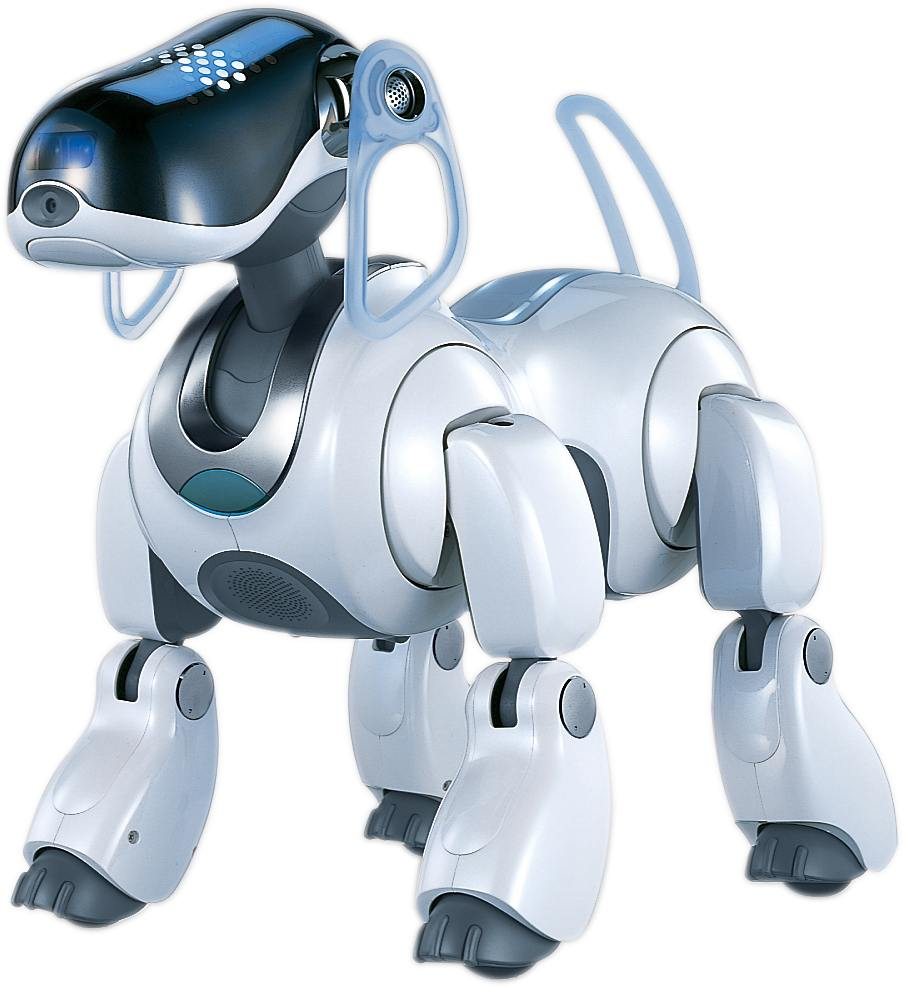
\includegraphics[scale=0.1]{Imatges/ERS7.jpg} 
\end{figure}

Cal indicar la titulació, que és un TFG, l'Escola.
Realment es pensa canviar tota la portada i agafar la que està penjada a la pàgina d'ETSEIB que és la que s'ha d'entrega, aquesta es tan sols provisional.

\newpage
\paragraph{}
\thispagestyle{empty}
\cleardoublepage

\setcounter{page}{1} %Començar en la pagina 1

\begin{abstract}
\addcontentsline{toc}{section}{Resum}
L'estabilitat del robots...
\end{abstract}

\renewcommand{\abstractname}{Resumen}
\begin{abstract}
\addcontentsline{toc}{section}{Resumen}
La estabilidad de los robots...
\end{abstract}

\renewcommand{\abstractname}{Abstract}
\begin{abstract}
\addcontentsline{toc}{section}{Abstract}
The estability of the robots...
\end{abstract}
\newpage
\cleardoublepage

\tableofcontents
\newpage
\listoffigures
\newpage
\listoftables
\newpage


%\printglossary
%\newpage

\section*{Prefaci}
\addcontentsline{toc}{section}{Prefaci}
\label{Prefaci}


\subsection*{Motivació}
\addcontentsline{toc}{subsection}{Motivació}
\label{Motivacio}

\paragraph{}A moltes persones que tenen devoció pel món de la robòtica, aquesta els hi ha vingut des de ben joves; aquest no és el meu cas. A mi m'agradava la informàtica. Essent un escolar vaig aprendre de forma autodidacta a programar en \textit{C++} i crear un servidor propi. Fet que ajudà, en arribar a la \textit{UPC}, a divertir-me amb assignatures relacionades amb programació, però em faltava veure reflectit el meu treball amb alguna utilitat física. No va ser fins que a l'assignatura de ``Projectes II'' vam controlar un mecanisme a través d'un microcontrolador \textit{Arduino}\footnote{\textit{Arduino} és la marca d'una família de microcontroladors.}, amb programació basada en \textit{Wiring} \cite{Arduino}, que vaig veure clar cap on volia enfocar el meu futur, la robòtica.

D'aquesta motivació, que ha crescut poc a poc, n'ha sorgit el perquè de desenvolupar aquest \textit{TFG} (\textit{\textbf{T}reball \textbf{F}inal de \textbf{G}rau}). A més, a cada pas que he fet en el treball, com més he vist i entès la gran complexitat d'altres robots, com el \textit{Big Dog} de \textit{Boston Dinamics} o el \textit{NAO} d'\textit{Aldebaran Robotics}\footnote{En l'estat de l'art es dona una breu explicació d'aquests i altres robots.}, entre d'altres, més estímuls tenia per avançar i millorar.

Ara bé, deixant de banda les pròpies ganes de treballar en robòtica, també he tingut en compte la preparació pel futur professional. Per això, en molts casos, a l'hora de fer alguna elecció, he intentat escollir la que fos més innovadora i útil en un futur proper. Aquest fet es visualitza tant en l'elecció dels llenguatges de programació utilitzats, com també en l'algorisme de resolució de la problemàtica de treball en qüestió. Per tant, queda palès que aquest treball té com a motivació la combinació d'entusiasme pel món de la robòtica, la millora continuada d'un mateix per tal de poder arribar a un bon futur professional en aquest camp i l'objectiu d'integrar els coneixements i habilitats apresos al llarg del grau.


\subsection*{Definició del \textit{TFG}}
\addcontentsline{toc}{subsection}{Definició del \textit{TFG}}
\label{Definicio-del-TFG}

%Amb un o dos paràgraf definir que és exactament el que s'intenta aconseguir: Utilitzant el robot AIBO, que es troba sobre una plataforma mòbil, el robot ha de ser capaç a reaccionar al moviment de la plataforma de tal manera que aconseguesqui una posició més adequada a tal objectiu de no caure.
%Tambe dir que aquest projecte forma part d'un conjunt en que s'intenta dur a terme un proces de reutilització dels AIBOs que des de fa un temps estan practicament en total desús


\subsection*{Requeriments previs}
\addcontentsline{toc}{subsection}{Requeriments previs}
\label{Requeriments}

\paragraph{}Per fer el seguiment del \textit{TFG} que es presenta, tot i que s'ha intentat donar explicació als conceptes que podrien ser més complicats d'entendre, és necessari disposar d'uns certs coneixements previs o nocions en \textit{ROS} (per \textit{\textbf{R}obot \textbf{O}perative \textbf{S}ystem})\footnote{S'explica detalladament en l'apartat \ref{ROS}.}, Control Automàtic, llenguatge de programació \textit{Python}, Mecànica i Xarxes de dades.

A banda del que s'ha esmentat anteriorment, per reproduir de nou l'experiència és molt recomanable llegir articles sobre aprenentatge de robots, tant per reforç, com utilitzant \textit{DMPs} (per \textit{\textbf{D}ynamic \textbf{M}ovement \textbf{P}rimitives}). Algunes devles referències més recomanades es poden trobar a l'apartat de Referències o Bibliografia.

Finalment, el més necessari de tot és tenir molta motivació i paciència, per així, no decaure davant les adversitats que un s'arriba a trobar i continuar endavant.

\newpage

\section{Introducció}
\label{Introduccio}

\paragraph{}Els robots són mecanismes programables i accionats per dos o més eixos amb cert grau d'autonomia, movent-se en el seu entorn, per realitzar les tasques previstes \cite{ISO_Robot}. Actualment, els robots s'utilitzen principalment a nivell industrial, per la realització d'accions de forma més exacte i barata o per treballs perillosos o repetitius. Ara bé, també existeix el cas de robots com l'AIBO, de Sony, entre d'altres robots, que poden ser utilitzats tant per entreteniment de l'usuari, com robot social o per la investigació o millora dels robots actuals.

Els estudis en robòtica es poden centrar tant en el \textit{hardware}, com en el \textit{software}. Tot i només enfocar-se en una de les dues branques, sempre es requereix de l'altre en més o menys proporció. El fet és que el dissenyar i fabricar el \textit{hardware} necessari s'emporta una gran partida del pressupost. Per això, en les investigacions que no compten amb grans pressuposts, com ara estudis universitaris, és comú l'ús de robots comercials en que es pot modificar el codi intern, com és el cas de l'AIBO.

A banda d'aquest robot, n'hi ha molts més que són utilitzats per dur a terme investigacions, tant robots comercials, com dissenyats i fabricats des de zero. El treball present es centra en l'AIBO, l'estabilitat, el modelat i l'aprenentatge d'un robot, per tant, tan sols es fa l'estudi d'antecedents d'aquests casos.


\subsection{Objectius}
\label{Objectius}

%S'han de posar un objectius quantificables, de tal manera que el tribunal pugui valorar com de bé s'han aconseguit. Estil adaptar-se fins a certs graus de pendent de la plataforma, temps de resposta, implementar ROS, implementar DMPs, implementar aprenentatge per reforç, fer un model, utilitza sistemes de filtratge per l'entrada de dades de l'acceleròmetre, 
\paragraph{}L'objectiu principal del present \textit{TFG} és l'optimització de l'adaptabilitat d'un robot quadrúpede, en aquest cas l'AIBO, a plans inclinats desconeguts pel robot. Per arribar a aquest objectiu s'han hagut de marcat uns objectius més concrets:
\begin{itemize}
\item Dissenyar un entorn de treball complert que permeti que l'algorisme utilitzat pugui ser processat en l'ordinador i enviar la informació necessària de forma remota a l'AIBO. En aquest cas l'entorn de treball tal que permeti això és el \textit{ROS}.
\item Utilització de l'algorisme més adequat, tenint en compte tant l'entorn del robot i ell mateix, com l'abast del treball. Per això s'haurà de fer un estudi dels diferents mètodes existents que podrien ser útils per l'objecte del treball.
\item Dur a terme una fase d'aprenentatge pel robot. Per poder fer-ho, abans, s'haurà d'haver fet un estudi en profunditat del aprenentatge per reforç.
\item Realització de diferents proves per comprovar el correcte funcionament. Tant per poder comprovar, com per fer la fase d'aprenentatge del robot, és necessita d'una plataforma mòbil que en aquest cas ja està construïda, pel Carlos Ramos (estudiant de l'\textit{EPSEVG}) \cite{TFG_Carlos_Ramos}, però s'ha de millorar per fer-la més robusta.
\end{itemize}



\subsection{Planificació}
\label{Planificacio}

\subsubsection{Planificació inicial}


\subsubsection{Planificació final}


\subsection{Pressupost}
\label{Pressupost}



\subsection{Metodologia}
\label{Metodologia}
%Dir que s'ha intentat implementar els fets més novedosos avui dia a la robotica, com és en el control de robots les DMPs o amb la comunicacio amb aquest el ROS, també esta molt a l'ordre del dia l'ús d'algorismes d'aprenentatge per això s'ha plantejat el supervisat i el pel reforç i s'ha cregut convenient crear un model per tal de millorar tant l'aprenentatge com el control d'un mateix a banda de prevenir davant possibles riscos que porta el fer-ho amb el robot físic.
%Es basa en crear una trajectoria inicial de demostracio, per a cada articulació, que té com a posició final una depenent de la inclinació del propi robot. A partir d'aquesta s'apren la DMP, això vol dir extreure uns pesos per unes funcions gaussianes. En tenir apreses la DMPs, es pot modificar la inclinació del robot, al canviar aquest, el goal de cada articulacio (que té cadascun una DMP) es veu modificat segons quina articulació sigui i la inclinació, i el robot s'adapta en temps real a aquesta modificació de la pendent.
%El que és voldria mirar d'aconseguir és prenent la solució anterior com a solució inicial, i millorar-ne els pesos i el goal amb l'algorisme PI^2, aquest pot prendre com a paràmetre influent algun que sigui extern al propi sistema dinàmic, com en aquest cas podria ser la pendent del robot, intentant que aquest estigui horitzontal, que requereix d'un aprenentatge per reforç i per tant a base de prova i error es milloren els pesos i el goal.


\subsection{Abast del treball}
\label{Abast}


\subsection{Estat de l'art}
\label{Estat-de-l'art}

%cercar articles o memories que utilitzin robots i que siguin sobre estabilitat tant sigui de quadrupedes, bipedes com de Zero Moment Point
%També cercar sobre com tractar el tema del centre de gravetat (COG)
%I també parlar de les referencies dels diferents Learnings

%Diferents plataformes mobils

\paragraph{}En la branca d'investigació sobre l'estabilitat en robots, tant bípedes, com quadrúpedes, hi ha multitud de tesis, treballs, articles, etc. Tots ells, centrant-se en un o altre aspecte com són: el punt de moment zero (\textit{ZMP}, per \textit{\textbf{Z}ero \textbf{M}oment \textbf{P}oint}), modelat de robots, aprenentatge supervisat, per reforç o \textit{DMP}, generador de patrons centrals (\textit{CPG}, per \textit{\textbf{C}entral \textbf{P}attern \textbf{G}enerator}), algorismes genètics (\textit{GA}, er \textit{\textbf{G}enetic \textbf{A}lgorithms})\footnote{La majoria d'aquests conceptes seran explicats al llarg d'aquest apartat.}, i molts altres.

Tot seguit, s'exposa un conjunt d'antecedents, organitzat en diferents àmbits, importants tots ells tant per realitzar l'experiència, com per entendre els factors que han conduït a cadascuna de les decisions preses.


\subsubsection{Robot AIBO}
\label{AIBO}

\paragraph{}L'AIBO (\textit{\texttt{A}rtificial \texttt{I}ntelligence Ro\texttt{BO}t}) és un robot quadrúpede dissenyat i fabricat per Sony Corporation, amb aparença canina. El primer model, que va ser tret al mercat, fou el \textit{ERS-110} l'any 1999, a partir d'aquest, i després de tres generacions, el 2003 s'arribà al \textit{ERS-7}, molt més sofisticat que els seus predecessors, tot i que en el 2006 s'aturà la producció de la família AIBO. L'\textit{ERS-7} és el model que s'estudia i s'utilitza en el present treball.

Aquest és considerat un robot autònom, per tant, és capaç d'extreure informació del seu entorn, funcionar per un període llarg sense la intervenció humana, moure alguna o totes les parts d'ell mateix dins d'un entorn de treball sense l'ajut d'un humà i, finalment, evitar situacions de perill per les persones, els bens o ell mateix, si no és per especificacions del propi disseny.

L'aplicació d'aquest robot autònom està enfocada en ser utilitzat en propòsits d'entreteniment, tot i ser, en molts casos, utilitzat en tasques d'investigació. Els robots autònoms corrents tendeixen a ser dissenyats per desenvolupar tasques de seguretat o treballs perillosos, ara bé, en aquests casos no es pot tolerar cap tipus d'error en les operacions crítiques. Mentre que si estan dissenyats per usos d'entreteniment, en el cas que es produís algun error no seria un amenaça per la vida \cite{Fujita2000}.

Els dissenyadors de l'AIBO han perseguit l'objectiu d'aconseguir que el comportament sigui el més realista possible, que sembli viu. Per assolir-ho, han avançat per diferents camins:
\begin{itemize}
\item Estímuls
\begin{itemize}
\item Comportaments reflexius i deliberats segons una escala de temps.
\item Comportaments per ordres externes i per desigs interns (instints i emocions).
\item Motivacions independents donades per parts del robot com coll, cua i potes.
\end{itemize}
\item Instints i emocions amb els que pot canviar el comportament davant d'altres estímuls externs.
\item Aprenentatge i evolució, inicialment és com un nadó sense pràcticament cap coneixements. Així com passa el temps, l'AIBO aprèn i creix segons com el tractis. Per tant, podria arribar a comportar-se com un noi entremaliat, si no se li dona l'atenció necessària.
\end{itemize}

%REVISAR TOTALMENT ES TEMA DE TAULES I FIGURES!!!!


\vspace{20pt}
\textbf{\textit{Hardware}}
\label{Hardware}

Les característiques del robot són les següents: \cite{Anshar2007}

\begin{itemize}
\begin{minipage}[t]{\textwidth}

\begin{wrapfigure}{r}{0.52\textwidth}
                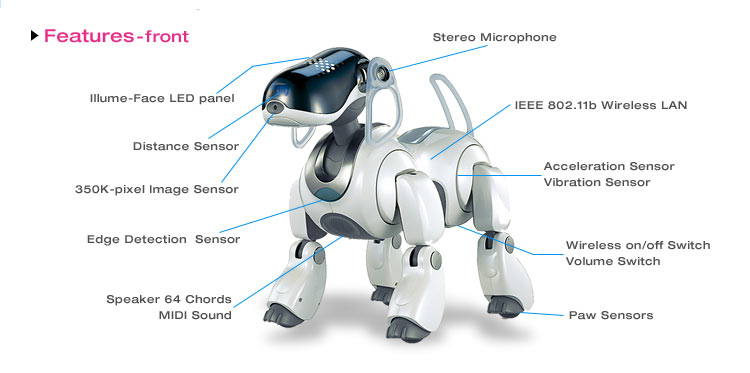
\includegraphics[width=0.5\textwidth]{Imatges/ERS-7(front)}
                \caption{AIBO ERS-7 (vista frontal) \cite{Aibo_Images}}
\end{wrapfigure}
\item Processador MIPS R7000 de 576 MHz 
\item Memòria \textit{RAM} de 64 MB
\item \textit{LAN} sense fils, 802.11b (estàndard)
\item Targeta interna de memòria lectura/escriptura 
\item 18 articulacions \textit{PID}, cadascuna amb un sensor de força
\begin{itemize}
\item 4 potes
\begin{itemize}
\item 3 articulacions cadascuna (elevació, rotació i genoll)
\item 1 sensor de pressió a cada peu
\end{itemize}
\item 3 articulacions al coll (moviment horitzontal, vertical i inclinació)
\item 2 articulacions a la cua (moviment vertical i inclinació)
\item 1 articulació a la boca
\end{itemize}
\end{minipage}

\begin{minipage}[t]{\textwidth}
\begin{wrapfigure}{r}{0.52\textwidth}
                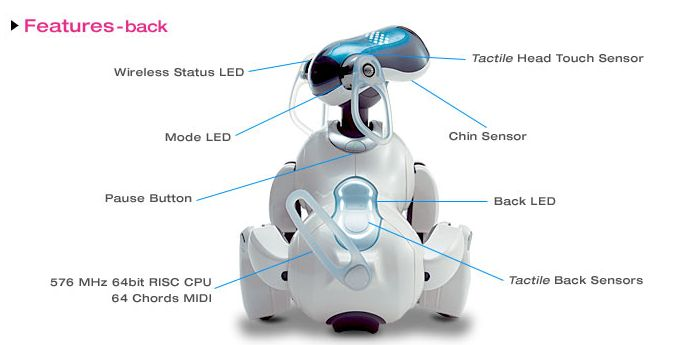
\includegraphics[width=0.5\textwidth]{Imatges/ERS-7(back)}
                \caption{AIBO ERS-7 (vista posterior) \cite{Aibo_Images}}
\end{wrapfigure}

\item 2 orelles, on hi ha els micròfon estèreo i amb una articulació booleana (posició dalt o baix)
\item Altaveus de 500 mW
\item 26 LEDs independents
\item Càmera de vídeo
\begin{itemize}
\item Sensor d'imatge CMOS
\item 56.9$^{\circ}$ ample i 45.2$^{\circ}$
\item Resolucions: $208\times160, 104\times80, 52\times40$
\item 30 imatges per segon
\end{itemize}
\end{minipage}

\begin{minipage}[t]{\textwidth}
\begin{wrapfigure}{r}{0.52\textwidth}
        			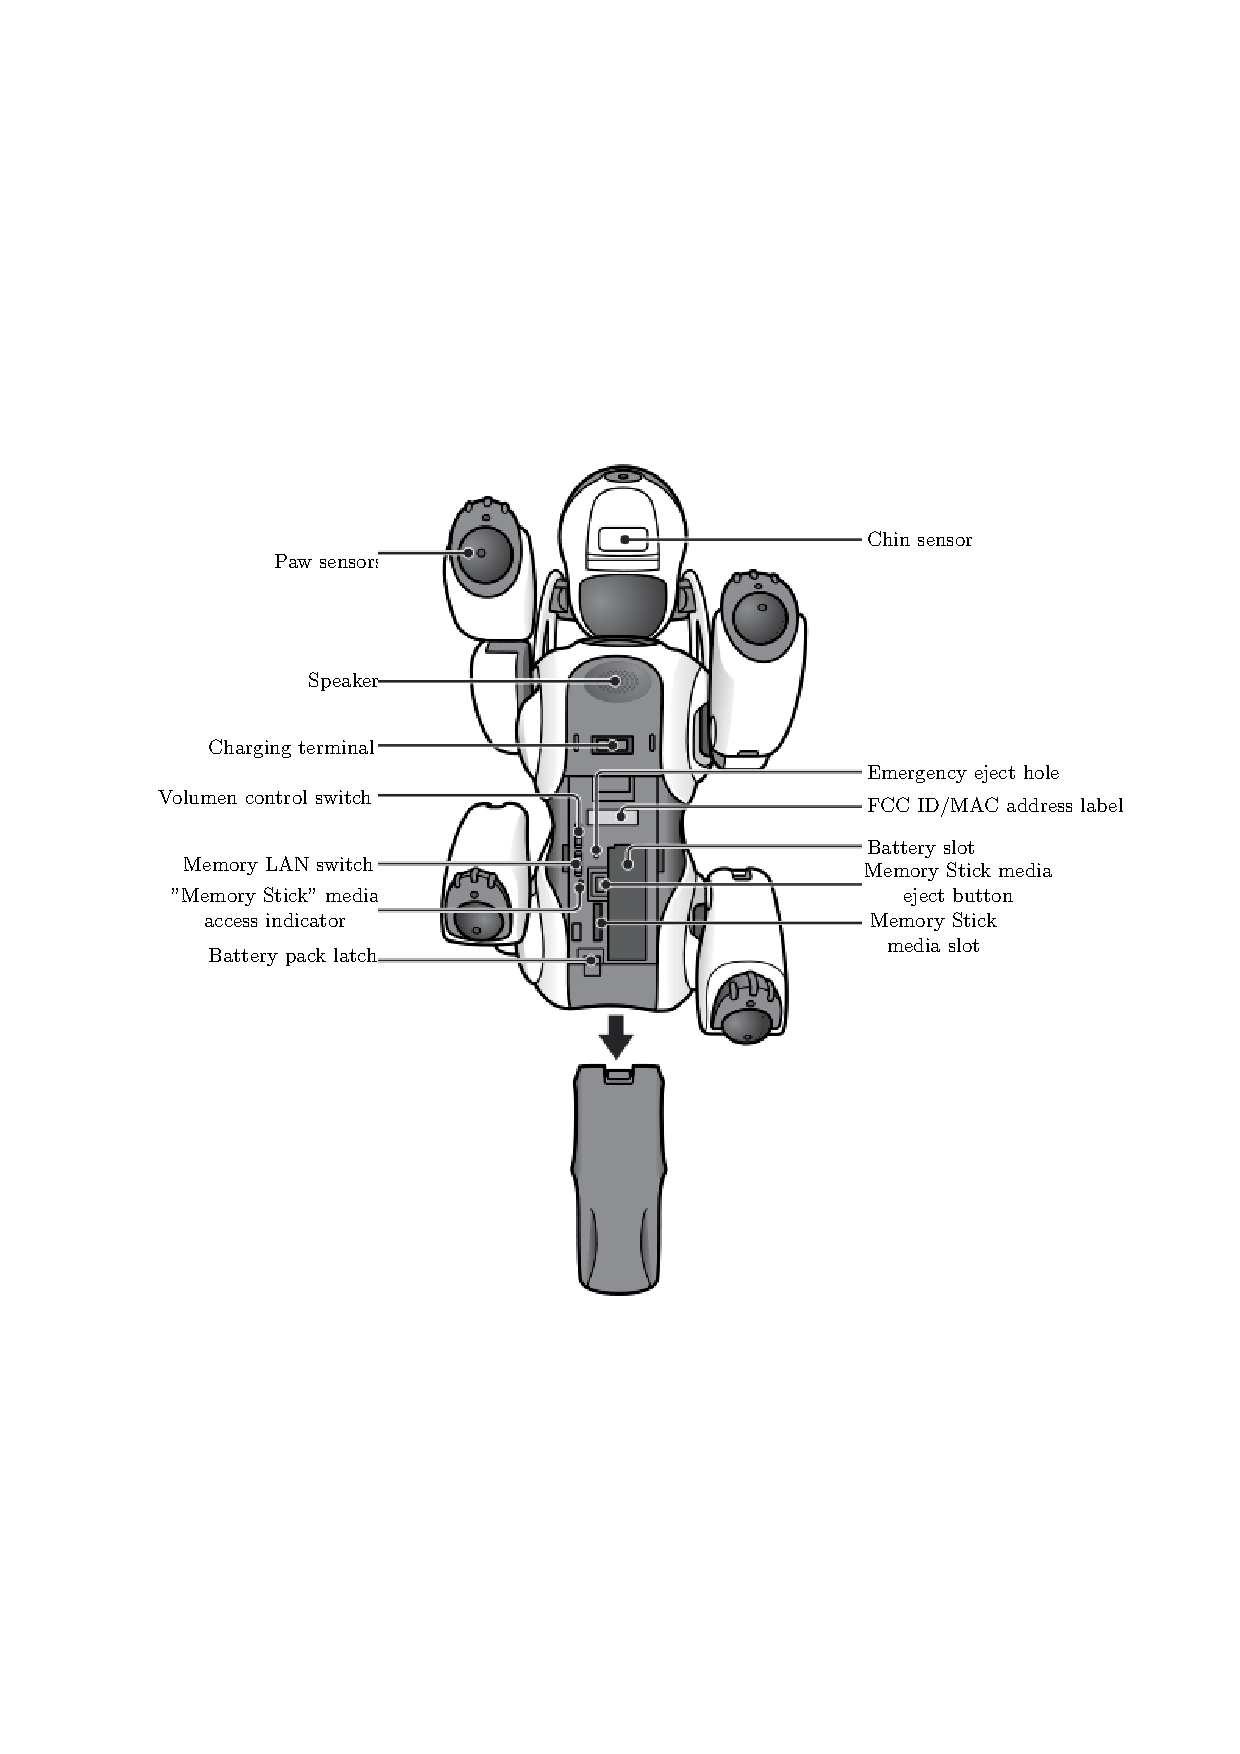
\includegraphics[width=0.5\textwidth]{Imatges/ERS-7(stomach)}
                \caption{AIBO ERS-7 (vista inferior) \cite{Aibo_Images}}
\end{wrapfigure}
\item 3 sensors de distància per infrarojos (un al cos i dos al nas, d'aquests dos, un és per objectes llunyans i un altre per pròxims)
\item Acceleròmetres \textit{X}, \textit{Y} i \textit{Z}
\item 4 botons sensorials de pressió (un al cap i tres al llom)
\item 1 botó booleà sota la boca
\item Sensor de vibració
\item Actualització dels sensors cada 32 ms, amb 4 mostres per actualització
\item Dimensions: $319\times180\times278$
\item Pes aproximat: 1,65 kg (bateria i targeta de memòria incloses)
\end{minipage}
\end{itemize}


Les articulacions \textit{PID}, segons la seva funció i les pròpies limitacions físiques tenen uns rangs de treball diferents, aquest són els que s'exposen tot seguit: 

\begin{table}[h]
\begin{center}
\begin{tabular}{| c | c | c | c |}
\hline
Name & Range & Units & Description\\ \hline \hline
legRF1    &    range=[-134.000000,120.000000]  & unit=deg & Right fore legJ1\\
legRF2    &    range=[-9.000000,91.000000]     & unit=deg & Right fore legJ2\\
legRF3    &    range=[-29.000000,119.000000]   & unit=deg & Right fore legJ3\\
legRH1    &    range=[-134.000000,120.000000]  & unit=deg & Right hind legJ1\\
legRH2    &    range=[-9.000000,91.000000]     & unit=deg & Right hind legJ2\\
legRH3    &    range=[-29.000000,119.000000]   & unit=deg & Right hind legJ3\\
legLF1    &    range=[-120.000000,134.000000]  & unit=deg & Left fore legJ1\\
legLF2    &    range=[-9.000000,91.000000]     & unit=deg & Left fore legJ2\\
legLF3    &    range=[-29.000000,119.000000]   & unit=deg & Left fore legJ3\\
legLH1    &    range=[-120.000000,134.000000]  & unit=deg & Left hind legJ1\\
legLH2    &    range=[-9.000000,91.000000]     & unit=deg & Left hind legJ2\\
legLH3    &    range=[-29.000000,119.000000]   & unit=deg & Left hind legJ3\\
neck      &    range=[-79.000000,2.000000]     & unit=deg & Neck tilt1\\
headTilt  &    range=[-16.000000,44.000000]    & unit=deg & Neck tilt2\\
headPan   &    range=[-91.000000,91.000000]    & unit=deg & Head pan\\
tailPan   &    range=[-59.000000,59.000000]    & unit=deg & Tail pan\\
tailTilt  &    range=[2.000000,63.000000]      & unit=deg & Tail tilt\\
mouth     &    range=[-58.000000,-3.000000]    & unit=deg & Mouth\\
\hline
\end{tabular}
\end{center}
\caption{Rangs de funcionament de les articulacions \cite{Urbi_Docs}}
\label{Taula-rangs-articulacions}
\end{table}

%Alguna solució per posar la taula al seu lloc
%\pagebreak funciona, però la pagina anterior amb queda amb un espai interlinial molt gran
%El mateix passa amb el parametre [H]



\vspace{20pt}
\textbf{\textit{Software}}
\label{Software}
%Quina versio d'Urbi és perque realment la comunicacio entre Urbi i ROS per versions posteriors ja existeix

%Que és OPEN-R, Tekkotsu, Urbi (aquest darrer hauria de ser de es qe es diu mes cosa pero tampoc sense preocupar-se)

%Com s'ha esmentat anteriorment, l'AIBO aprèn i evoluciona segons el seu entorn amb uns coneixements inicials quasi nuls. Però sí que incorpora unes funcions bàsiques, com ara, caminar, reconeixement de veu, reproducció de sons, entre moltes altres.


%Actualment, l'AIBO per defecte té multitud facultats, com ara, caminar en diferents direccions sense perdre l'equilibri o quedar-se en una posició de repòs estable, entre d'altres. Tot i que això només és possible en condicions òptimes (terreny pla i llis, sense forces externes que actuïn sobre el robot, etc.). Aquestes funcions i més ja han estat desenvolupades en llenguatges com OPEN-R o Tekkotsu (nivell mitjà) o Urbi (nivell alt). El repte és poder aconseguir fer això i més en ROS (\textit{Robot Operating System}), que proveeix un entorn de treball òptim per la creació de programari per a qualsevol robot, i per tant pot ser exportable de l'AIBO a qualsevol altre robot que compleixi els requisits mínims de \textit{hardware}.  
  


\subsubsection{\textit{ROS}}
\label{ROS}

\paragraph{}\textit{\texttt{R}obot \texttt{O}perating \texttt{S}ystem} \cite{ROS} és un entorn de treball \textit{open-source} i flexible per la programació de robots. Les bases d'aquest projecte s'iniciaren en unes investigacions a Stanford el 2007, on es varen dur a terme diferents prototips d'entorns de treball per programari de robots, com ara \textit{\textbf{ST}anford \textbf{A}rtificial \textbf{I}ntelligence \textbf{R}obot} (\textit{STAIR}) o \textit{\textbf{P}ersonal \textbf{R}obotics} (\textit{PR}). Més endavant, \textit{Willow Garage}, una empresa inversora en robòtica, va proveir recursos per tal de millorar el concepte i permetre crear implementacions correctament testejades. Finalment, amb la col·laboració desinteressada d'incomptables investigadors, millorant el nucli de \textit{ROS} i les eines principals que proveeix, s'ha arribat al que és ara, una plataforma àmpliament utilitzada en les investigacions de robòtica.

En el moment de la redacció d'aquest treball, la versió més actual de \textit{ROS} és la \textit{ROS Hydro Medusa}, publicada el setembre de 2013, i pròximament es publicarà la \textit{ROS Indigo Igloo}. La Hydro està dissenyada especialment per Ubuntu 12.04 LTS (\textit{Precise}), tot i suportà també altres sistemes Linux, Mac OS X, Android i Windows en altres graus.


\vspace{20pt}
\textbf{Estructura de \textit{ROS}}

\textit{ROS} ofereix una interfície que permet la comunicació entre processos per tal de processar dades conjuntament, és comú referir-s'hi com a capa intermèdia. Els conceptes fonamentals de la implementació de \textit{ROS} són els \texttt{nodes}, \texttt{Master}, \texttt{messages}, \texttt{services}, \texttt{topics} i \texttt{bags}.

\begin{itemize}
\item \textbf{Nodes}: Els \texttt{nodes} són processos que realitzen càlculs. Típicament, un sistema compren multitud de \texttt{nodes}. En aquests casos és útil entendre les comunicacions entre \texttt{nodes} com un graf, amb arcs que uneixen els que s'estan comunicant.

\item \textbf{Master}: El \textit{ROS} \texttt{Master} proveeix els noms d'enregistrament dels \texttt{nodes}, \texttt{topics} i \texttt{services} existents als altres \texttt{nodes}. Per tant, el \texttt{Master} rep la informació de registre dels \texttt{nodes} i després aquest informa als altres \texttt{nodes} per tal que puguin establir, entre ells, connexions de forma adequada. 

\item \textbf{Messages}: Els \texttt{nodes} es comuniquen un amb l'altre mitjançant \texttt{messages}. Aquest són simplement estructures de dades, que poden anar des de tipus \texttt{integer}, \texttt{float}, \texttt{boolean} fins a \texttt{array}.

\item \textbf{Topics}: Un \texttt{node} envia un \texttt{message} mitjançant la publicació d'aquest en un \texttt{topic} donat. El \texttt{topic} és el nom que s'utilitza per identificar el contingut d'un \texttt{message} concret. 

\item \textbf{Services}: El \texttt{service} és el nom que ha d'utilitzar un \texttt{node} per enviar un \texttt{message}, amb la funció de sol·licitar una resposta que depèn del \texttt{message} enviat.

\item \textbf{Bags}: Els \texttt{bags} són un format per guardar i poder reproduir un altre cop les dades de \texttt{messages} de \textit{ROS}. Aquests són de gran importància a l'hora d'emmagatzemar dades i, per tant, per desenvolupar i testejar algorismes.
\end{itemize}

Aquesta capa intermèdia ofereix dos models de comunicació: (1) sistema de \textit{publicació/subscripció} (\texttt{publisher}/\texttt{subscriber}) ; i (2) utilitzant \texttt{services}.

\begin{enumerate}

\item El sistema de \textit{publicació/subscripció} és anònim, asíncron i les dades poden ser capturades i rellegides sense canvis en el codi. Per tant, si per fer una certa tasca es requereix de les dades d'una altra tasca, com per exemple un sensor, llavors a partir de subscriure's al \texttt{topic} corresponent es poden llegir les dades que publica la tasca (sensor). Pot haver-hi múltiples publicadors i subscriptors per un únic \texttt{topic} i, en general, entre ells no saben de l'existència dels altres.

\item Els \texttt{services} estan definits per dos \texttt{messages}, un és la demanda que ha fet el \texttt{node} i l'altre és la resposta a aquesta demanda. Per tant, el seu ús és molt simple, en el moment que es crida un \texttt{service}, amb les dades que aquest requereixi, el procés dona una resposta al \texttt{node} segons les dades que s'han enviat.
\end{enumerate}


\vspace{20pt}
\textbf{Objectius de \textit{ROS}}

El principal objectiu de \textit{ROS} és poder \textit{reutilitzar} el codi de desenvolupament i d'investigacions en robòtica. L'estructura de processos distribuïts permet aquest fet, ja que pot executar-se un procés (amb un codi determinat) de forma individual i acoblar-se fàcilment al conjunt. A més, aquests processos poden agrupar-se en \texttt{Packages} i \texttt{Stacks}, per ser compartits de forma senzilla.

D'altra banda, també és tenen altres finalitats \cite{Quigley}: (1) descentralització; (2) plurilingüisme; (3) estar basat en eines; (4) ser una capa intermèdia fina; (5) gratuïta i \textit{open-source}.

\begin{enumerate}

\item Descentralització

\textit{ROS} està estructurat de forma que els processos estan distribuïts, amb la possibilitat de trobar-se en \textit{hosts} diferents, però funcionant conjuntament. Altres entorns de treball, que poden també treballar amb múltiples processos i \textit{hosts}, si es basen en un servidor central, podrien tenir problemes en una xarxa heterogènia\footnote{Una xarxa heterogènia és una xarxa de connexió d'ordinadors i altres dispositius amb diferents sistemes operatius i/o protocols \cite{Delphinanto2011}.}.

\item Plurilingüisme

Cada programador és un món, cadascú té el seu llenguatge de programació preferit, sigui per la raó que sigui. Per això, \textit{ROS} s'ha dissenyat per ser un llenguatge neutral. Actualment, \textit{ROS} admet quatre llenguatges de programació: (1) \textit{C++}, (2) \textit{Python}, (3) \textit{Octave} i (4) \textit{LISP}, havent altres en desenvolupament.

\item Basat en eines

S'ha optat per dissenyar un nucli simple, on s'utilitzen multitud d'eines per construir i fer funcionar els diversos components de \textit{ROS}, en lloc, de dissenyar un enorme entorn de treball, tot en un. Tot i haver-se implementat alguns serveis en el propi nucli, s'ha intentat distribuir tot en mòduls separats. La pèrdua d'eficiència compensa els guanys en estabilitat i complexitat del conjunt.

\item Capa intermèdia fina

En molts casos, és molts difícil ``\textit{extreure}'' la funcionalitat d'un codi, del seu context original, per a poder ser reutilitzat, això és degut a factors provocats pel propi entorn de treball d'origen. Per això, en \textit{ROS} s'indueix a la independència dels algorismes, amb el nucli del \textit{ROS}, creant-los en llibreries separades. Es facilita l'extracció de codi i la seva reutilització a traves d'aquest fet, entre d'altres característiques de la interfície.

\item Gratuït i \textit{open-source}

El codi natiu de \textit{ROS} està disponible públicament. Aquest és un fet que permet facilitar el testeig i correcció de \textit{software} en tots els nivells. 

\end{enumerate}

\vspace{20pt}
\textbf{Eines de \textit{ROS}}

Com s'ha comentat breument en l'apartat anterior, \textit{ROS} és basa, en gran part, en la multitud d'eines que disposa. Aquestes eines poden arribar a dur a terme diverses tasques diferents, per exemple, navegar per l'arbre de codi font, obtenir i establir els paràmetres de configuració, visualitzar les connexions entre processos, mesurar la utilització d'ample de banda, exposar de forma gràfica les dades dels \texttt{message}, i més. A continuació es comenten breument alguns dels més utilitzats:
\begin{itemize}
\item \texttt{rviz}\\
\texttt{rviz} és un entorn de visualització 3D que pot combinar les dades dels sensors del robot i el model que es té, juntament amb altres dades 3D que se li aporti, per poder visualitzar el conjunt.

\item \texttt{rosbag} i \texttt{rxbag}\\
\texttt{rosbag} és la comanda que et permet emmagatzemar i reproduir de nou les dades d'un \texttt{message} en un arxiu \texttt{bag}. Per altra banda, \texttt{rxbag} és un visualitzador per a les dades emmagatzemades dins els arxius \texttt{bag}.

\item \texttt{rxplot}\\
\texttt{rxplot} permet veure dades escalars publicades en els \texttt{topics} de \textit{ROS}.

\item \texttt{rxgraph}\\
\texttt{rxgraph} exposa visualment amb un gràfic com funcionen els processos de \textit{ROS} i les seves connexions, en aquell instant.

\end{itemize}

%Afegir apartat de packages i messages d'interés (per tal d'explicar l'actionlib, dmp, sensor_msgs.msg (JointState), control_msgs.msg (FollowJointTrajectoryGoal, FollowJointTrajectoryAction), trajectory_msgs.msg (JointTrajectoryPoint) i altre que es puguin trobar)
%http://docs.ros.org/api/sensor_msgs/html/msg/JointState.html
%http://docs.ros.org/api/control_msgs/html/action/FollowJointTrajectory.html
%http://docs.ros.org/api/trajectory_msgs/html/msg/JointTrajectoryPoint.html

%Fins ara no s'ha donat suport oficial a AIBO en ROS...
%topics que té l'AIBO actualment
%Ricardo Téllez


\subsubsection{Robots}
\label{Robots}

%Afegit fotografies de cada un dels robots
\paragraph{}Alguns dels robots sobre els que s'hi ha investigat, amb temàtiques relacionades amb el treball present són:
\begin{description}
\item[QRIO]
\begin{minipage}[t]{0.94\linewidth}
Robot humanoide dissenyat i fabricat per Sony Corporation, és el successor de l'AIBO. Entre d'altres articles i investigacions que se n'ha fet es troba \cite{Nagasaka2004} sobre l'estabilitat d'un robot bípede a l'hora de caminar, córrer i saltar. Basat en la teoria del \textit{ZMP}.
\end{minipage}

\item[REEM-C]
\begin{minipage}[t]{0.94\linewidth}
	\begin{wrapfigure}{r}{0.3\textwidth}
	    \centering
		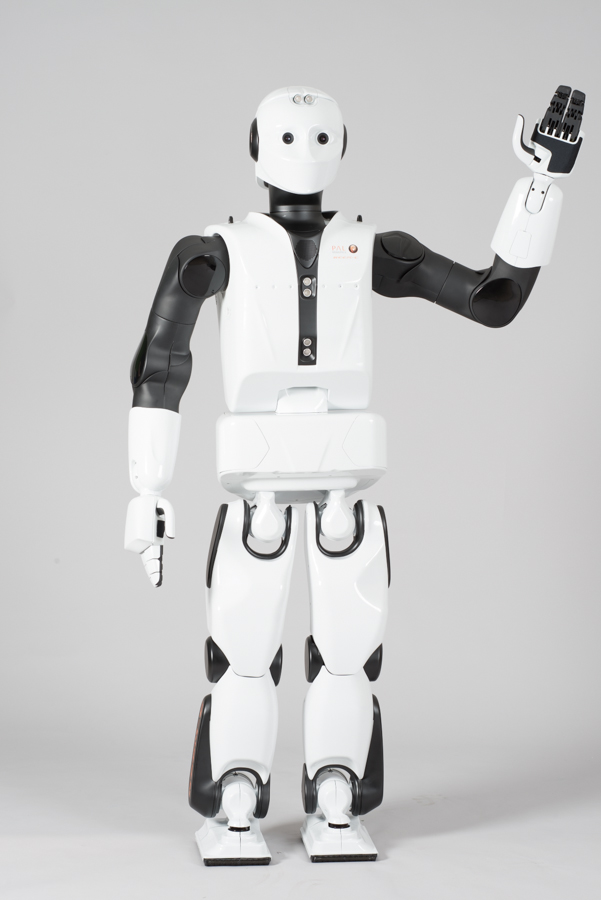
\includegraphics[width=0.22\textwidth]{Imatges/REEM-C}
                \caption{REEM-C \cite{REEM_C}}
     \end{wrapfigure}
Aquest humanoide és el creat per PAL Robotics \cite{REEM_C}. Destaca pel fet de ser el primer bípede enfocat en la investigació i basat 100\% en \textit{ROS}. El REEM-C està basat, entre d'altres teories, en el \textit{ZMP} i en l'aprenentatge propi del robot. A més, les seves característiques de reconeixement de veu, manipulació d'objectes i d'interacció amb humans, és una eina educativa molt útil \cite{REEM_C}.
\end{minipage}

\paragraph{}$ $%PER AJUSTAR TEXT

\item[ASIMO]
\begin{minipage}[t]{0.94\linewidth}

És un altre robot humanoide, aquest desenvolupat per HONDA, a partir de l'any 2000. Inicialment, en els seus predecessors, tan sols s'havia plantejat el fet de crear un robot mòbil bípede, però, poc a poc, s'hi han incorporat més facultats, fins arribar a ser un dels humanoides amb els moviments més semblants al dels humans \cite{ASIMO_History}. De les referències llegides en el moment de redactar el treball, de l'ASIMO hi ha estudis sobre la planificació dels passos per tal d'evitar obstacles \cite{Chestnutt2005} i sobre la interacció amb els humans \cite{Mutlu2006}.
\end{minipage}\\

%ARREGLAR TEMA DE MINIPAGE QUE PROVOCA QUE ELS PEUS DE PAGINA ESTIGUIN MAL POSATS!!!

\item[BigDog]
\begin{minipage}[t]{0.94\linewidth}
	\begin{wrapfigure}{r}{0.3\textwidth}
	    \centering
		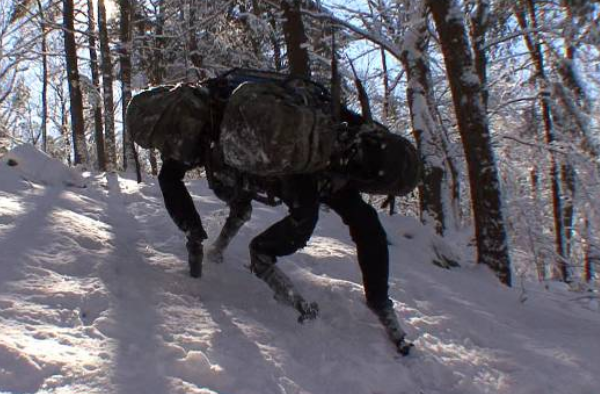
\includegraphics[width=0.30\textwidth]{Imatges/BigDog}
                \caption{BigDog \cite{Raibert2008}}
	\end{wrapfigure}
És un dels grans robots que s'han creat a l'empresa \textit{Boston Dynamics}, prenent el que va ser inicialment desenvolupat en la \textit{DARPA} \cite{Raibert2008}. Aquest ``\textit{gos}'' va ser dissenyat per ús militar, en concret, per acompanyar als soldats portant la càrrega necessària en terrenys on no podria desplaçar-se un vehicle convencional. Aquest quadrúpede és dinàmicament estable\footnote{Sistema que és estable tenint en compte els efectes inercials i altres components dinàmiques que apareixen en el propi sistema \cite{Purushotham2009}.} gràcies al gran conjunt de sensors i actuadors que arriba a tenir. A banda d'un sistema mecànic molt complert, també s'hi ha implementat algorismes d'aprenentatge per reforç (\texttt{Reinforcement Learning}\footnote{Aprenentatge per reforç s'explica en detall en l'apartat \ref{RL-estat-de-l'art}. En molts casos es abreviat com \textit{RL}.}), en concret \textit{DMP} (\textit{\textbf{D}ynamic \textbf{M}ovement \textbf{P}rimitives})\footnote{\textit{DMP} (\textit{\textbf{D}ynamic \textbf{M}ovement \textbf{P}rimitives}) s'explica en detall en l'estat de l'art a l'apartat \ref{DMP-estat-de-l'art}. } \cite{Raibert2008}.
\end{minipage}

\item[LittleDog]
\begin{minipage}[t]{0.94\linewidth}
	\begin{wrapfigure}{r}{0.32\textwidth}
	    \centering
		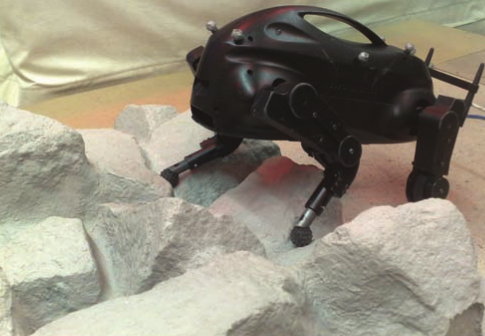
\includegraphics[width=0.30\textwidth]{Imatges/LittleDog}
                \caption{LittleDog \cite{Kalakrishnan2010}}
     \end{wrapfigure}
 Aquest quadrúpede és el predecessor del BigDog. Té la mateixa base que l'anterior, tot i que en aquest és on s'ha fet més estudi del aprenentatge del robot. La investigació que s'hi ha fet al damunt, tant d'aprenentatge, com de criteri de \textit{ZMP} és pot entendre de forma genèrica en \cite{Kalakrishnan2010}. 
\end{minipage}\\

\end{description}

%\paragraph{}$ $%PER AJUSTAR TEXT

A banda dels nombrats anteriorment, existeixen molts altres robots amb potes que han servit per aprofundir en coneixements diversos, com l'estabilitat o l'aprenentatge dels robots. Molts d'ells han sigut creats des de zero, com són els següents exemples: (1) el PLEO, un robot ``\textit{dinosaure}", que en el projecte \cite{Menendez2011} se li aporta una millora substancial en la comunicació robot-ordinador; (2) el BISAM, on en l'article \cite{Albiez2003} s'estudia com provocar que els moviments siguin més semblants als d'un mamífer quadrúpede; (3) el MRWALL-SPECT IV, on l'autor d'aquests articles \cite{Loc2010} i \cite{Loc2011} es centra en l'adaptabilitat del quadrúpede a diferents terrenys; (4) el MERO, estudiat en \cite{Ion} per fer una anàlisi d'estabilitat quan aquest es desplaça; (5) per últim, també hi ha els casos d'hexàpodes, tant per l'estudi del caminar amb el criteri de les tres potes \cite{Lee1988}, com en la construcció des de zero \cite{Lojo2009}, entre d'altres. 


\subsubsection{Modelat de robots}
\label{Modelat de robots}

\paragraph{}Un model d'un robot és un sistema virtual que representa de forma aproximada la cinemàtica i/o la dinàmica d'un robot, mitjançant formes geomètriques enllaçades entre elles amb una configuració determinada. Aquesta és la base d'un model, ara bé, se li poden afegir complements, com un aspecte visual més vistós, amb alguna textura o concretar quins són els actuadors o sensors, on situar-los, etc.

Durant molt temps, per utilitzar un robot es requeria d'un model. D'aquesta manera, l'autòmat podia saber en quina posició es trobava, en tot moment, i reaccionar de forma correcte. Si no es feia seguint aquest procediment, l'única opció era que el programador tingués en compte totes les diferents possibilitats de fallada i les corregís, sent aquesta un tasca molt complicada.  

Per crear el model d'un robot existeixen diverses possibilitats. La més rudimentària és prenent les mesures del propi robot i introduir-les al programa, avui dia aquest mètode és poc utilitzat quan es vol un model molt acurat. El més típic, en aquests casos, és utilitzar el propi robot, amb una arquitectura d'aprenentatge òptima, per fer el model. Aquesta arquitectura es basa en un sistema realimentat amb (1) robot, (2) el model en construcció i (3) un controlador per la realimentació; per així arribar finalment a desenvolupar el model,  està il·lustra molt clarament a la Figura \ref{fig:esquema-arquitectures-models}.

Ara bé, existeixen tant diferents tipus de models, com també formes diferents de crear-los segons \cite{Nguyen-Tuong2011}:

\begin{itemize}
\item Tipus de models:

\begin{description}

\item[Directes] Aquest preveu el pròxim estat d'un sistema dinàmic, donada un acció i estat actual. Per tant, els models directes representen la relació causal entre estats i accions. Una de les seves utilitats és en el control automàtic clàssic, entre d'altres.

\item[Indirectes] Per altra banda, aquests preveuen l'acció requerida pel sistema per passar d'un estat actual al desitjat pel futur. A diferència dels directes, aquest representen una relació anticausal. Aquest és molt utilitzat en estudis de dinàmica inversa, ja que la relació inversa està ben definida.

\item[Mixtes] La combinació dels dos models dona el model mixt. La idea és que la informació del model directe pugui ajudar en la manca d'unicitat del model indirecte, ja que el model indirecte té infinitat de solucions. 

\item[De predicció de múltiples passos] Finalment, aquest és principal utilitzat per la predicció d'una acció o estat futur concret, sense la disponibilitat de les mesures en del moment en qüestió.

\end{description}

\paragraph{}Cadascun dels models té unes característiques que el defineixen, però aquestes delimiten els diferents modes d'aprenentatge que poden ser utilitzats per crear-los. Per tant, no tots els models poden ser creats a partir de qualsevol arquitectura d'aprenentatge. Aquest fet s'exemplifica a la Taula \ref{T_model-arquitectura}.

\end{itemize}

\begin{table}[tb]
\begin{center}
\begin{tabulary}{\textwidth}{|C|C|}
\hline

\multirow{2}{*}{\textbf{Model Type}}
& \textbf{Learning} \\ 
& \textbf{Architecture} \\ \hline \hline

\multirow{1}{*}{Forward Model}
& Direct Modeling\\ \hline

\multirow{2}{*}{Inverse Model}
& Direct Modeling\\ 
& Indirect Modeling\\ \hline

\multirow{4}{*}{Mixed Model}
& Direct Modeling \\
& (if invertible) \\
& Indrect Modeling \\
& Distal-Teacher \\ \hline

\multirow{1}{*}{Multi-step Prediction Model}
& Direct Modeling \\ \hline
\end{tabulary}
\end{center}
\caption{Relació tipus de model amb arquitectura d'aprenentatge \cite{Nguyen-Tuong2011}\label{T_model-arquitectura}}
\end{table}

%\paragraph{} %Per crear una separació entre text i taula

\begin{itemize}
\item Arquitectura d'aprenentatge:
\begin{description}

\item[Modelat directe] El model s'extreu a partir d'aprendre de l'observació dels \textit{inputs} i els \textit{outputs} del propi robot. Aquesta és probablement la tècnica d'aprenentatge més freqüent per aproximació de models.

\item[Modelat indirecte] Una de les tècniques per dur a terme modelat indirecte és l'aprenentatge de l'error de realimentació. Aquest utilitza l'error creat pel controlador de realimentació per tal d'aprendre i crear així el model. 

\item[Aprenentatge amb professor distal] La idea és crear un model invers, però guiat amb un model directe, per tal de minimitzar la manca d'unicitat del model invers.  

\end{description}

\end{itemize}

\begin{figure}[tb]
\begin{center}
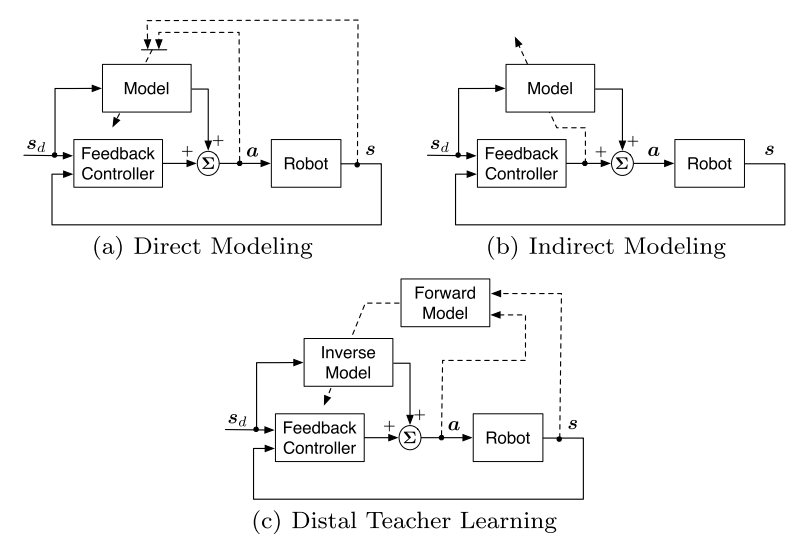
\includegraphics[scale=0.5]{Imatges/arquitectures-d'aprenentatge.png}
\caption{Esquema de cada arquitectura d'aprenentatge \cite{Nguyen-Tuong2011}\label{fig:esquema-arquitectures-models}}
\end{center}
\end{figure}


Un dels beneficis de tenir el model d'un robot és poder fer simulacions virtuals del robot, de tal manera que no es provoca cap desgast al robot real, ni es poden donar situacions de perill. Tot i ser de gran utilitat, els simuladors també tenen les seves limitacions, és difícil simular la física d'un robot (actuadors, interaccions amb l'entorn, sensors\dots) de manera realista. A més, passar de simulacions a un robot real no sempre és fàcil \cite{Hohl2006}.

Ara bé, existeixen una gran multitud de simuladors cada un amb les seves peculiaritats. Alguns dels que s'ha pogut extreure informació i que podrien ser de més interès són els següents:

\begin{description}
\item[Webots\texttrademark] \cite{Michel2004} Simulador de robots mòbils desenvolupat per Cyberbotics Ltd. La física està basada en Open Dinamic Engine (\textit{ODE}), per així simular una dinàmica més acurada. Aquest \textit{software} proveeix un entorn de treball per modelar i programar el teu propi robot, a més inclou models de diversos robots com són Sony AIBO, Khepera, Lego Mindstorms\texttrademark o Pioneer2. Però té la desventatge que és un simulador de pagament.

\item[SimRobot] \cite{Laue2006a} Aquest és un simulador genèric de robots en 3D. Com el Webots\texttrademark , el SimRobot també es basa en la física d'\textit{ODE}. Un dels inconvenients d'aquest simulador és que no es possible transferir els controladors de la simulació al robot real.

\item[Gazebo] \cite{Khatib2002} És un simulador multi-robots en 3D. Aquest, al igual que Webots\texttrademark , permet el modelat del teu propi robot, tot i ser en llenguatge C. També es diferencia pels models de robot que inclou, que són el Pioneer2DX i el SegwayRMP.
\end{description}

Com s'ha mencionat, Webots\texttrademark inclou un model del Sony AIBO, dissenyat en \cite{Hohl2006}. Aquest té implementat l'estructura cinemàtica, propietats dinàmiques\footnote{Masses i moments d'inèrcia.}, el seu control i l'aspecte gràfic. Per altra banda, també es poden simular els sensors de distància i els de les potes. El model té certes limitacions, els sensors del llom, cap, acceleròmetres i tèrmics no estan implementats per poder ser simulats. 


\subsubsection{Aprenentatge supervisat \textit{(SL)}}

\paragraph{}En l'aprenentatge supervisat (en estadística anomenat \textit{anàlisi clúster}), un agent extern presenta una sèrie de dades d'exemple o d'entrenament, que són prediccions correctes a fer en diferents situacions \cite{Kober2009}. A partir d'aquestes dades d'entrenament, s'ha d'extreure un model estadístic per tal que, en una situació desconeguda, s'esculli l'acció correcte. L'aprenentatge supervisat és, segons \cite{Cord2008}, la metodologia més important d'aprenentatge automàtic i amb molt pes en el processament de dades multimèdia.

Les dades a estimar poden ser binàries, on s'escull si una dada desconeguda és d'un tipus (p. e. pertany a un grup o no), o numèriques, on s'utilitza la regressió per aproximar. Tant siguin unes o altres, les bases de l'aprenentatge supervisat són: (1) el model estadístic, (2) la funció de pèrdua i la d'error d'aproximació, i (3) procediment d'optimització \cite{Alpaydin2004}.

\begin{enumerate}

\item El model es representa com $g(x|\theta)$\footnote{La $x$ són les entrades, mentre $\theta$ són els paràmetres.}, on \textit{g}(·) és la classe d'hipòtesi i els valors de $\theta$ donen una hipòtesi en concret, d'entre les possibles en el model.

\item La funció de pèrdua, \textit{L}(·), quantifica la diferència entre la sortida desitjada, $r^t$, i l'aproximació $g(x^t|\theta)$, mentre la suma de les pèrdues de cada cas és l'error d'aproximació 

\begin{equation} \label{eq:er-aprox}
E(\theta|X)=\sum_{t} L(r^t,g(x^t|\theta))
\end{equation}

\item El procediment d'optimització per trobar $\theta^*$ que minimitza l'error total, $E(\theta|X)$, és:

\begin{equation} \label{eq:theta-opt}
\theta^*=arg\,\operatorname*{min}_\theta E(\theta|X)
\end{equation}

En models complexes, seria més convenient utilitzar mètodes basats en el gradient (p. e. gradient descendent, gradient conjugat, gradient biconjugat\dots) o l'algorisme de recuita simulada\footnote{A partir d'una solució inicial es selecciona una nova, aleatòriament, pròxima a la inicial. Si es millor s'hi queda, i sinó, segons una certa probabilitat, torna a l'anterior o es queda en la nova. Això es repeteix fins a la condició d'acabament\cite{Torrent-Fontbona2013}.}.

\end{enumerate}

Un dels algorismes més simples és la classificació per veí més proper, aquest és molt útil per entendre el funcionament bàsic de l'aprenentatge supervisat \cite{Learned-Miller2014}. En aquest cas, les dades d'entrenament estan etiquetades, per tant, cada una pertany a un grup en concret. Suposem que es té alguna forma de fer el càlcul de la distància entre dues mostres $x_{1}$ i $x_{2}$, expressat com $D(x_{1}, x_{2})$.

Llavors amb la forma simplificada, pel cas de binàries, de \eqref{eq:theta-opt}
\begin{equation} \label{eq:theta-opt-exemple}
i^*=\operatorname*{arg\,min}_{i\in\{1\dots n\}} D(x_{t}, x_{i})
\end{equation}

Sent $x_{t}$ la dada a classificar i $x_{i}$ l'exemple més pròxim. Després de trobar $i^*$, s'assigna l'etiqueta de $x_{i}$ a $x_{t}$, queda així classificada la dada. Per suposat, aquesta assignació és una suposició, pot ser correcte o incorrecte.


\subsubsection{Aprenentatge per reforç \textit{(RL)}}
\label{RL-estat-de-l'art}

\paragraph{}En la robòtica, l'aprenentatge per reforç proveeix d'unes eines molt útils per tal de crear comportaments sofisticats i amb gran dificultat de disseny. Permet a un robot desenvolupar el seu propi comportament a base de prova i error. En aquest cas, el dissenyador, en lloc de donar unes dades per explícitament crear la solució al problema, tan sols proveeix una realimentació amb una funció objectiu de valors escalars que mesura la bondat de l'acció anterior. Per tant, un agent explora les possibles estratègies i després rep una recompensa per l'acció feta, intentant sempre maximitzar la recompensa acumulada durant el seu temps de vida \cite{Kober2009}. Però a diferència de l'aprenentatge supervisat, no es ``\textit{diu}"  quina acció hauria estat la millor a llarg plaç, a més de no haver d'explorar l'entorn, una altra diferència, en \textit{RL} el fet de les accions ser en temps real és molt influent, ja que és concurrent amb l'aprenentatge \cite{Kaelbling1996}. 

Aquest agent i el seu entorn poden ser modelat com un estat\footnote{Un estat $s$ conté la informació necessària per descriure la situació actual i futures.}  $s\in S $ i una acció\footnote{Un estat del sistema es controlat o carregat per una acció $a$.}  $a \in A$. Una recompensa es donada a l'agent, per cadascuna de les accions que desenvolupa, en funció de l'estat i les observacions. L'objectiu de \textit{RL} és crear una política\footnote{Per política s'entén com en \cite{iec-dlc} ``\textit{Manera de conduir un afer.}''} $\pi$ que maximitza la recompensa acumulada escollint unes accions $a$ en determinats estats $s$.

La idea clàssica d'aprenentatge per reforç es prenia des del punt de vista que l'agent consistia en un procés de decisions de Markov (\textit{Markov Decsion Process} o \textit{MDP})\footnote{Conjunt d'estats $S$, accions $A$, recompenses $R$ i probabilitats de transició T, aquest últim defineix la dinàmica del sistema per predir l'efecte de l'acció en un estat donat.} on la propietat de Markov estableix que el següent estat $s'$ i la recompensa estan definits tan sols per l'acció $a$ i l'estat $s$ \cite{Sutton1998}. %Actualment, no tots els estudis que es fan segueixen el concepte de \textit{MDP}, ja que s'utilitza el \texttt{RL} sense tenir definit el sistema dinàmic, per tant, sense saber l'efecte de l'acció sobre l'estat. 

%S'hauria de posar la parta comentada anteriorment? Tot i que del sistema dinamic només se'n parla en el peu de pagina?

L'acumulació de recompensa és el que es maximitza o minimitza segons l'algorisme utilitzat, aquí s'exemplifica maximitzant. Per tant segons el mètode d'atorgar la recompensa es defineix el comportament òptim \cite{Kober2009}. Existeixen diversos models, aquí se n'exposen tres:
\begin{description}


\item[Horitzó finit] Aplicat en models on es sap en quants passos es resol el problema, maximitza la recompensa per \textit{H} passos.
\begin{equation}
J=E\left\{ \sum_{h=0}^{H} R_{h} \right\}.
\end{equation}

\item[Model de descompte] Un factor de descompte ($\gamma\in[0,1)$) a la recompensa futura. Aquest és introduït manualment i determina en quina proporció afecta el futur\footnote{Com més pròxim a 0 la recompensa a llarg plaç és menys significant, ara bé, també s'ha de tenir en compte que la \textit{policy} òptima pot ser inestable si el factor de descompte és massa baix \cite{Kober2009}.}.
\begin{equation}
J=E\left\{ \sum_{h=0}^{\infty} \gamma^h R_{h} \right\}.
\end{equation}

\item[Recompensa mitja] Finalment en aquest es té en compte la mitja total de les recompenses. El problema d'aquesta és que no es pot diferenciar si s'esta afavorint l'inici o el final del temps de vida.
\begin{equation}
J=\lim_{H \to \infty} E\left\{ \frac{1}{H}\sum_{h=0}^{H} R_{h} \right\}.
\end{equation} 

\end{description}

A l'hora d'estimar la política $\pi$ òptima, existeixen una gran diversitat de mètodes que es podrien desglossar en dos grans grups segons si requereixen del model probabilístic de transició T$(s',a,s)$.

\begin{itemize}

\item Els mètodes que requereixen de model són anomenats \textit{model-based}.

\item Per altra banda, dels que no requereixen d'un model els més utilitzats són el \textit{Monte Carlo}, Mètodes de diferencia temporal, \textit{SARSA}, \textit{R-learning} i \textit{Q-learning}, sent aquest últim el més extès, gràcies a la seva senzillesa.

\end{itemize}

El comportament aprés és totalment depenent de la funció de recompensa que s'ha utilitzat. En la practica, és molt difícil crear la funció per a l'aprenentatge per reforç d'un robot. En molts cops, convé utilitzar recompenses contínues per tal de guiar l'aprenentatge, en lloc d'una recompensa binària segons si s'ha complert o no la tasca \cite{Laud2004}. Molts cops el comportament no és l'esperat, tot i que, per la nostra forma de pensar semblés que la solució és òbvia. Per això, en alguns casos, s'utilitza l'aprenentatge per reforç invers, que aconsegueix extreure la funció recompensa gràcies a un seguit de demostracions, pot ser no sigui la verdadera recompensa, però provoca l'actuació de la forma desitjada \cite{Kober2009}.

Alguns dels molts problemes que comporta el fet d'aplicar-se en robots es descriuen a \cite{Kober2009}. A banda d'haver de decidir la forma de treballar: com d'acurat es vol el control del robot, si discret o per aproximació de funcions, a quina freqüència actuar, etc. Un ha de tenir en compte que l'augment de la dimensionalitat provoca un creixement exponencial dels càlculs per cobrir l'espai d'estats i accions, és per això que en molts cops es treballa l'aprenentatge de forma jeràrquica\footnote{S'assumeix que una part és fixa, mentre les altres s'aprenen, per tenir un solució inicial per després fer l'aprenentatge global.} o amb tasques progressives\footnote{Alguns cops és més senzill aprendre una tasca complicada si es fan anteriorment algunes de no tant complicades.}. 
Per altra banda, dur a terme experiments en el món físic és car, la comunicació i reacció dels motors del robot porten sempre un cert retard, pot ser complicat el recrear les condicions de l'entorn necessàries per l'aprenentatge i s'ha de tenir molta cura perquè l'exploració d'aquest entorn sigui segur, ja que pot crear tot tipus de riscs. Per a molts d'aquests problemes, la solució podria ser l'ús de models simulats, però s'ha de tenir en compte que aquests no són perfectes i tan sols un petit error pot acumular i donar un comportament diferent.

\subsubsection{\textit{DMP} (\textit{\textbf{D}ynamic \textbf{M}oviment \textbf{P}rimitive})}
\label{DMP-estat-de-l'art}

\paragraph{}Les \textit{DMPs} representen un moviment a partir d'un conjunt d'equacions diferencials, on la dinàmica del propi sistema corregeix les pertorbacions que puguin aparèixer, és per això que són considerats sistemes robusts davant pertorbacions. A més, és molt fàcil modificar l'objectiu (o \textit{goal}) del moviment al estar presentat com equacions, ja que tan sols és modificar el paràmetre \textit{g} en l'equació . Aquesta robustesa i adaptabilitat que dona aquest tipus d'entorn de treball és molt favorable per millorar altres sistemes d'aprenentatge com és l'aprenentatge per demostració (\textit{learning from demostration} o \textit{LfD}) on a partir de certs exemples s'aprén el comportament.

El \texttt{LfD} és podria estructurar en tres grans grups, segons la forma d'adquirir les dades de la demostració:
\begin{description}

\item[Imitació] L'exemple és produeix sobre una plataforma que no és el robot, per tant, la informació extreta requereix ser modificada i interpretada per adequar-se a les articulacions del robot. Dos possibles mètodes són amb sensors a sobre el professor o a través de l'observació externa amb els sensors del robot.

\item[Demostració] L'execució és produeix sobre el mateix robot, per tant, no s'han de transformar les dades per tal d'interpretar com és el moviment sobre els motors del propi robot. En aquest cas, un dels mètodes utilitzats és la teleoperació del robot per part del professor, mentre l'autòmat registre el moviment amb els sensors propis.

\item[Trajectòria programada] Per últim, la demostració pot ser donada per un seguit de coordenades d'una trajectòria preestablerta en el propi codi. Aquest cas, només es possible d'efectuar si el robot "\textit{sap}" en tot moment la posició de les seves articulacions, i per tant, és pot complir perfectament el recorregut. 

\end{description}

El sistema dinàmic és pot interpretar com un PD\footnote{Controlador proporcional i derivatiu.}, amb els paràmetres \textit{K}, pel coeficient proporcional, i \textit{D}, pel derivatiu; o com si fos un sistema mecànic de molla lineal amb una força externa viscosa, en aquest cas, sent el coeficient de fregament i de la fricció viscosa respectivament. Per últim, la \textit{x} i \textit{v} són la posició i la velocitat, la constant $\tau$ és el període del moviment i \textit{g} és el paràmtre d'atracció del sistema.

\begin{align}
\tau \dot{v} &= K(g - x) - Dv + (g - x_0)f(s)\label{eq:tau-v-dot-DMP}\\
\tau \dot{x} &= v\label{eq:tau-x-dot=v}
\end{align}

Si s'estudia el sistema dinàmic unidimensional de les equacions \eqref{eq:tau-v-dot-DMP} \eqref{eq:tau-x-dot=v}, que correspondrien al sistema de transformació (\textit{transformation system}), és pot comprovar que aquest és estable, tendint sempre a la posició \textit{g}, per qualsevol valor de $f(s)$. Aquesta és una funció no lineal que no depèn del temps, sinó de la variable de fase $s\in [0,1]$ que representa la durada del moviment en tant per un. Aquesta variable està definida per $\tau$ i per $\alpha$\footnote{La $\alpha$ és una constant pre-definida} com es veu en l'equació diferencial \eqref{eq:canonical-system}, conegut com a sistema canònic (\textit{canonical system}). A més, aquesta funció $f(s)$ pot aprendre per tal de dur a terme moviments complexes de forma arbitrària, ja que els pesos $w_i$ es poden ajustar.

\begin{align}
f(s) &= \frac{\sum_i w_i \psi_i(s)s}{\sum_i \psi_i(s)} \\
\tau \dot{s} &= - \alpha s \label{eq:canonical-system}
\end{align}

Les $\psi_i(s)$ són funcions gaussianes expressades com $\psi_i(s)=exp(-h_i(s-c_i)^2)$ on les $h_i$ defineixen l'amplada i les $c_i$ el centre de la gaussiana \textit{i}. La peculiaritat de la funció $f(s)$ és el fet de ser la suma ponderada de les gaussianes, cadascuna amb el seu pes, i per tant, pot crear la corba que és vulgui, com es veu exemplificat en la figura \ref{fig:gaussians-sum}. Això permet que, aquesta corba no lineal, sigui sumada amb la trajectòria, definida pels paràmetres \textit{K} i \textit{D}, com en l'exemple de la figura \ref{fig:DMP-with-gaussians}, per així, poder-se adaptar a noves situacions (com evadir obstacles, canvi d'objectiu, etc.).

\begin{figure}[tb]
\centering
\begin{subfigure}[h]{0.48\textwidth}
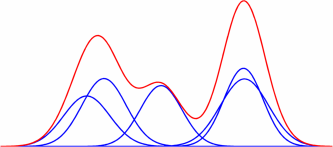
\includegraphics[width=\textwidth]{Imatges/gaussians-sum}
\caption{Representació de la suma de funcions gaussianes, on cada linea blava és una gaussiana i la vermella és la suma del conjunt \cite{Ruckert2012}.}
\label{fig:gaussians-sum}
\end{subfigure}
\begin{subfigure}[h]{0.48\textwidth}
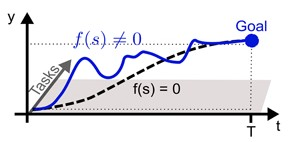
\includegraphics[width=\textwidth]{Imatges/DMP-with-gaussians}
\caption{Representació de la \textit{DMP} amb funció no lineal i sense \cite{Ruckert2013}.}
\label{fig:DMP-with-gaussians}
\end{subfigure}
\caption{Gràfics explicatius de la funció no lineal $f(s)$}
\end{figure}

Realment, en les \textit{DMPs}, el que determina la trajectòria duta a terme és la part no lineal, i aquesta es veu controlada per els pesos $w_i$. Per aprendre aquests existeixen diferents mètodes: (1) aprenentatge per demostració, on és fa una aproximació, per mínims quadrats, amb gaussianes d'aquesta trajectòria; (2) aprenentatge per reforç, en aquest cas, un dels algorismes més utilitzats per les \textit{DMPs} és el $\mathrm{PI^2}$, que s'explica en el següent punt d'aquesta secció.

\begin{figure}[tb]
\centering
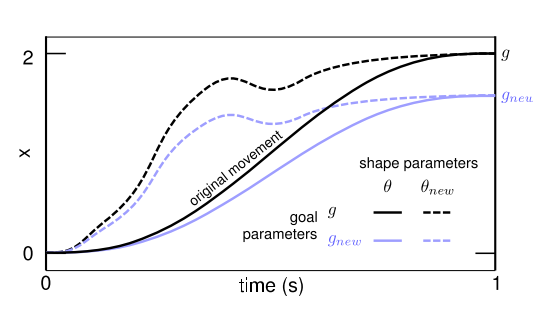
\includegraphics[width=0.8\textwidth]{Imatges/effect-of-shape-parameters}
\caption[Efecte dels pesos $w_i$ (representats per $\theta$) i de l'objectiu (\textit{goal})]{Efecte dels pesos $w_i$ (representats per $\theta$) i de l'objectiu (\textit{goal}) en la trajectòria \cite{Stulp2011}. Els pesos varien l'estil de la trajectòria, mentre el \textit{goal}, l'escurça o allarga.}
\label{fig:ffect-of-shape-parameters}
\end{figure}


Fins ara s'ha explicat l'algorisme original de les \textit{DMPs}, ara bé, aquest porta inherents una sèrie d'inconvenients \cite{Pastor2009}:

\begin{itemize}
\item Si la posició inicial $x_0$ i la posició \textit{g} són la mateixa, llavors la funció $f(s)$ no es capaç de desplaçar el sistema de l'estat inicial.

\item Si es dona el cas que $g-x_0$ és molt pròxim a zero, probablament $f(s)$ sigui un numero elevat, per tant, si varia el valor de \textit{g} pot provocar acceleracions molt grans que sobrepassi els limits del robot.

\item Finalment, s'ha de tenir en compte el fet que si el signe de $g_new - x_0$ és canviat respecte $g_{original} - x_0$ l'efecte de la funció no lineal és reflectit.
\end{itemize}

\begin{wrapfigure}{r}{0.55\textwidth}
\centering
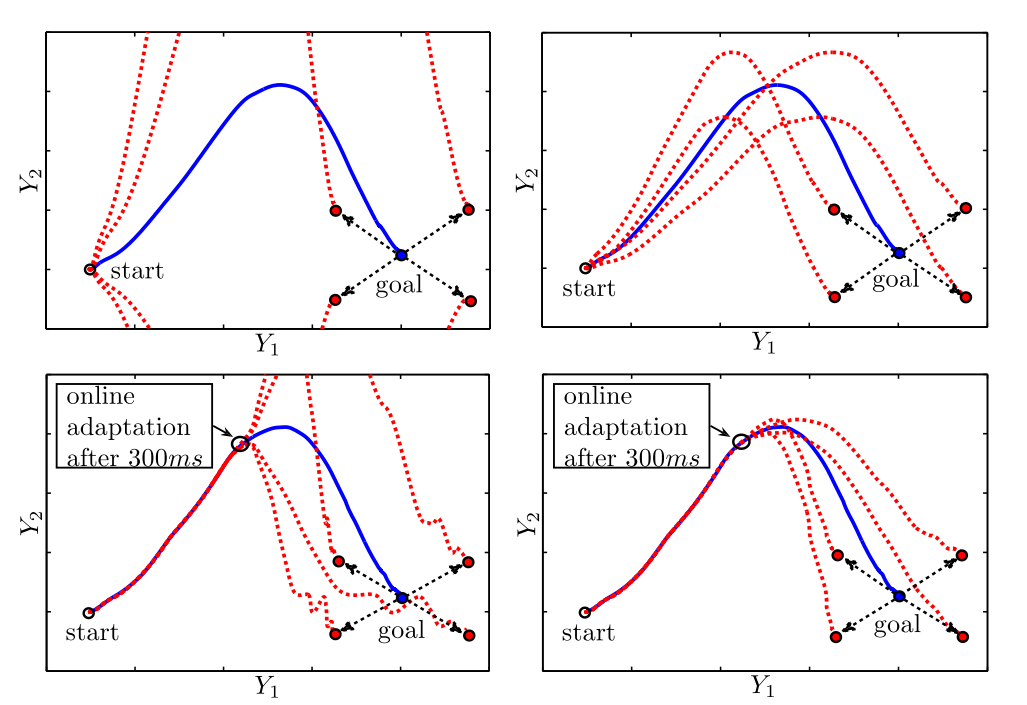
\includegraphics[width=0.55\textwidth]{Imatges/DMP-modified-algorism}
\caption[Comparació de l'algorisme de \textit{DMP} original (esquerra) i el modificat  per \cite{Pastor2009} (dreta)]{Comparació de l'algorisme de \textit{DMP} original (esquerra) i el modificat  per \cite{Pastor2009} (dreta). S'utilitzen els mateixos moviment original i \textit{goals}, a dalt els goals són modificats a l'inici, mentre a la part de baix es modifiquen als 300 ms d'haver començat.}
\label{fig:DMP-modified-algorism}
\end{wrapfigure}

Es per això, que en l'article \cite{Pastor2009} es proposa una modificació de l'algorisme original. L'única equació que es veu retocada és \eqref{eq:tau-v-dot-DMP} que és substituïda per
\begin{equation}\label{eq:tau-v-dot-DMP-modified}
\tau \dot{v} = K(g - x) - Dv - K(g - x_0)s + K f(s)
\end{equation}

Els trets importants són que $g - x_0$ no multiplica a $f(s)$ i el terme $K(g - x_0)s$ és necessari per tal que en l'inici del moviment no es produeixin salts, la millora, respecte l'algorisme original, es veu reflectida a la Figura \ref{fig:DMP-modified-algorism} de sobre.


\subsubsection{\textbf{P}ath \textbf{I}ntegral \textbf{P}olicy \textbf{I}mprovement ($\mathrm{PI^2}$)}

\paragraph{}L'algorisme $\mathrm{PI^2}$ \cite{Stulp2011} té com a principal objectiu polir el pesos $w_i$ (al llarg d'aquest apartat s'hi refereix com paràmetres $\theta_t$), per tal que es minimitzi la funció de cost \eqref{eq:PI2-cost-function} de la trajectòria $\tau_i$. Ara bé, una bona solució inicial, per aconseguir una convergència més ràpida, és l'extreta a partir del \texttt{LfD}, comentat en el punt anterior.

\begin{equation}\label{eq:PI2-cost-function}
J(\tau_i) = \phi_{t_N} + \int\limits_{t_i}^{t_N} (r_t + \frac{1}{2} \theta_t^T R \theta_t) \mathrm{d}t
\end{equation}

La funció $J(\tau_i)$ és creada per l'usuari, segons la tasca que es vulgui desenvolupar, sent $\phi_{t_N}$ el cost final, $r_t$ el cost immediat i $\frac{1}{2} \theta_t^T R \theta_t$ cost de control immediat\footnote{Regula el fet d'augmentar o disminuir els paràmetres $\theta_t$, envers el benefici de fer-ho \cite{Hennig2011}}. Aquests dos últims, determinen principalment els valors que prenen els diferents $\theta_t$ durant la trajectòria, mentre el cost final $\phi_{t_N}$ és el que decideix la bondat del resultat. Degut a la pròpia naturalesa d'aquests, el cost final ha de ser el més influent, ja que normalment el que interessa més és arribar a l'objectiu. Per això, quan la tasca que interessa és que en un determinat instant el robot passi per una coordenada en concret\footnote{Extret de \cite{Schaal2010} apartat 5.2 \textit{Learning Optimal Performance of a 1 DOF Via-Point Task}.}, els costos es presentarien d'una forma similar a \eqref{eq:funcio-costos-waypoint}. L'altre plantejament seria com un problema de \texttt{RL}, per exemple\footnote{Extret de \cite{Schaal2010} apartat 5.1 \textit{Learning Optimal Performance of a 1 DOF Reaching Task}.}, si es vol acabar en un punt (\textit{goal}), amb poca velocitat i durant el recorregut amb l'acceleració minimitzada seria de l'estil de \eqref{eq:funcio-costos-general}.

\begin{equation}
r_{300ms} = 100000000(G-y_{t_{300ms}})^2    \qquad {}  \phi_{t_N} = 0\label{eq:funcio-costos-waypoint}
\end{equation}

\begin{equation}
r_t = 0.5\ddot{y_t}^2 + \frac{1}{2}10000( \theta_t^T \theta_t)    \qquad {}  \phi_{t_N} = 10000(y_{t_N}^2 + (g-y_t)^2)\label{eq:funcio-costos-general}
\end{equation}

Els mètodes de millora de política, com és el $\mathrm{PI^2}$, consisteixen en un procés iteratiu d'exploració i actualització dels paràmetres. En l'exploració es proven $K$ \textit{DMPs} diferenciades per prendre els $\theta^{init}$ inicials més un cert soroll $\epsilon_{t,k}^{\theta}$, d'aquests se'n calcula les respectives funcions de cost i a partir d'aquí s'actualizen els valors dels paràmetres per donar $\theta^{new}$ que són els actuals.

\begin{figure}[tb]
\centering
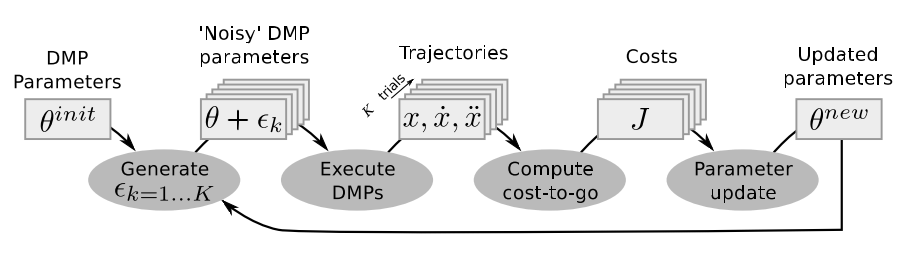
\includegraphics[width=0.5\textwidth]{Imatges/policy-improvement-loop}
\caption{Algorisme genèric dels mètodes de millora de política \cite{Stulp2011}}
\label{fig:policy-improvement-loop}
\end{figure}

Per últim, en el cas concret del $\mathrm{PI^2}$, l'algorisme segueix la següent estructura, segons \cite{Stulp2011} on està més detallat:

\begin{enumerate}
\item Determina el cost de cadascuna dels \texttt{trials}, per tant, du a terme cada \textit{DMP} amb el respectiu paràmetre $\theta^{init} + \epsilon_{t,k}^{\theta}$.

\item Calcula la probabilitat de cada un. La idea és que a menor cost, major probabilitat.

\item Proceix a calcular el $\delta\theta$, primer és traient la mitjana respecte els \texttt{trials}, on es té en compte la probabilitat d'aquests, i després la mitjana respecte el temps.

\item Finalment dona $\theta^{new} = \theta^{init} + \delta\theta$.
\end{enumerate}

\subsubsection{Algorismes avançats}

\begin{description}

\item[CPG] \textit{Central Pattern Generators}, la idea és crear una arquitectura capaç de generar coordinació entre diferents elements, independentment de la tasca a realitzar i de la plataforma robòtica utilitzada. Una forma de veure-ho és des del punt de vista dels autors de \cite{Tellez2005a}:
\begin{quotation}
"\textit{\dots we see the robot’s mind as a group of different modules each one in charge of its own device (sensor or actuator) that interacts with the rest of modules\dots} "
\end{quotation}

Aquesta cita podria ser traduïda com que cada dispositiu encarregant-se d'ell mateix, però amb la interacció amb els altres, tots junt arriben a crear la ment del robot.

Per poder dur a terme aquesta arquitectura es requereixen de dos tipus d'algorismes: (1) algorismes neuro-evolutius, per poder cooperar entre mòduls i controlar els elements associats; i (2) algorismes co-evolutius, per instruir i arribar a un objectiu comú entre tots.

%Necessari posar antecedents?? (\cite{Tellez2005a})
%using neural oscillators and Central Pattern Generators (CPG) [3][4][5][6], like for example the use of CPGs for the control of several postures and movements [7]

\item[CBR] \textit{Case Based Reasoning}, aquest algorisme podria ser considerat de la família de l'aprenentatge supervisat. Consisteix l'aproximació de l'acció correcte a través de dos tipus de dades: (1) dades d'entrenament, del mateix estil que les del supervisat; i (2) extretes a partir de la pròpia experiència. El cicle de funcionament del CBR seria el següent: (i) prendre el cas o els casos més semblants a la situació actual, dels que estan emmagatzemats; (ii) adaptar el cas pres a la situació; (iii) avaluar com de satisfactori ha estat la solució adoptada; (iv) aprendre d'aquest nou cas.

\item[GA] \textit{Genetic Algorithm}, és un mètode estocàstic de cerca que pren la idea de l'evolució biològica natural. Aquest pren uns antecedents aleatoris, d'aquests en treu solucions les quals s'hi provoca una mutació, per últim, les solucions alterades es converteixen en els antecedents. Aquest procés es repeteix fins arribar a la solució que s'adapta suficient a la funció objectiu o al limit de generacions.

\end{description}


\newpage

\section{Estudis preliminars}
\label{Estudis-preliminars}


\subsection{Comunicació mitjançant \textit{ROS}}
\label{ROS-estudi-pre}

%NO ES LA PRIMERA VEGADA, N'HI HA HAGUT D'ALTRES QUE HO HAN INTENTAT, NO A TRAVES D'URBI PERO PER ALTRES BANDES SI, mail de'n cecilio

\paragraph{}L'entorn de treball \textit{ROS} és una eina que està a l'ordre del dia en robòtica. Fins aquest moment, no existia la possibilitat de comunicació del robot AIBO a través de \textit{ROS}, tot i que han existit intents, però no serveixen pel nostre cas\footnote{Per una banda, el cas del \texttt{roseus package} \cite{Okada} que utilitza l'entorn de treball \texttt{EusLisp}, no ha tingut gaire èxit. Per l'altra banda, s'ha enfocat des de perspectives diferents, a les establertes en aquest treball, com en el cas de \cite{Rofer2013}.}. Per això, tot seguint una iniciativa del Departament d'Automàtica de la Universitat Politècnica de Catalunya, el doctor Ricardo Téllez va fer-se-la seva i va començar a crear un primer \texttt{package}. Des del Departament, i a través de diversos TFGs, s'ha promogut la continuació d'aquest \texttt{package} per permetre que l'AIBO pugui treballar amb \textit{ROS}. Per això, dos Projecte de Final de Carrera i aquest mateix Treball Final de Grau, han millorat de forma conjunta aquesta eina. Aquest ara permet la transferència de video i so, el control de les articulacions del robot, s'ha optimitzat la freqüència de treball, etc. 


\subsubsection{Entre l'AIBO i \textit{ROS}}

\paragraph{}El funcionament actual de la comunicació entre AIBO i \textit{ROS} es basa en Urbi, ja que la informació que es publica en els \texttt{topics} de \textit{ROS}, en realitat, són les dades extretes d'Urbi 1.5\footnote{S'ha de remarcar el fet que és l'Urbi 1.5 perquè per a versions posteriors ja existeix la comunicació entre Urbi i \textit{ROS}.}. De la mateixa manera, les accions de control que són publicades a \textit{ROS} s'interpreten i es transformen en comandes d'Urbi. Aquests conceptes s'expliquen a continuació en detall i es veuen il·lustrats en la Figura \ref{fig:Comunicacio-ROS-Urbi-AIBO}. Aquests dos tipus de tasques es desenvolupen en paral·lel per dos clients d'Urbi separats: (1) client publicador, és aquell que introdueix les dades de l'AIBO en els \texttt{topics}; (2) client subscriptor, on la seva funció és recollir el que s'ha publicat en el \texttt{topic} de comandes.

\begin{description}

\item[Publicació a \textit{ROS}] d'informació de l'AIBO a traves d'Urbi
\begin{enumerate}
\item Per una banda, Urbi demana la informació a l'AIBO, en forma de \texttt{callbacks}.
\item Per l'altra banda, Urbi publica continuament en els \texttt{topics}, on hi ha subscriptors, el missatge respectiu segons el \texttt{topic}.
\item En el moment en que la informació de l'AIBO és rebuda per Urbi, es modifica el missatge que aquest publica a \textit{ROS}.
\end{enumerate}

\item[Control de les articulacions] a partir d'un \texttt{topic}
\begin{enumerate}
\item L'algorisme de control crea un \texttt{topic} anomenat \texttt{aibo$\_$server$/$aibo$/$subJoints}, cada cop que s'hagi de modificar la posició de les articulacions, hi publica un \texttt{message}\footnote{El \texttt{message} conté un conjunt de \texttt{floats} que representen cadascuna de les articulacions, amb el seu nom seguint la Taula \ref{Taula-rangs-articulacions}, canviant la paraula ``\texttt{leg}" per ``\texttt{joint}".}.
\item En aparèixer un nou \texttt{message} al \texttt{topic}, Urbi pren el \texttt{message} i el transforma per tal d'enviar-lo com a comanda per les articulacions a l'AIBO.  
\end{enumerate}

\end{description}

\begin{figure}[tb]
\centering
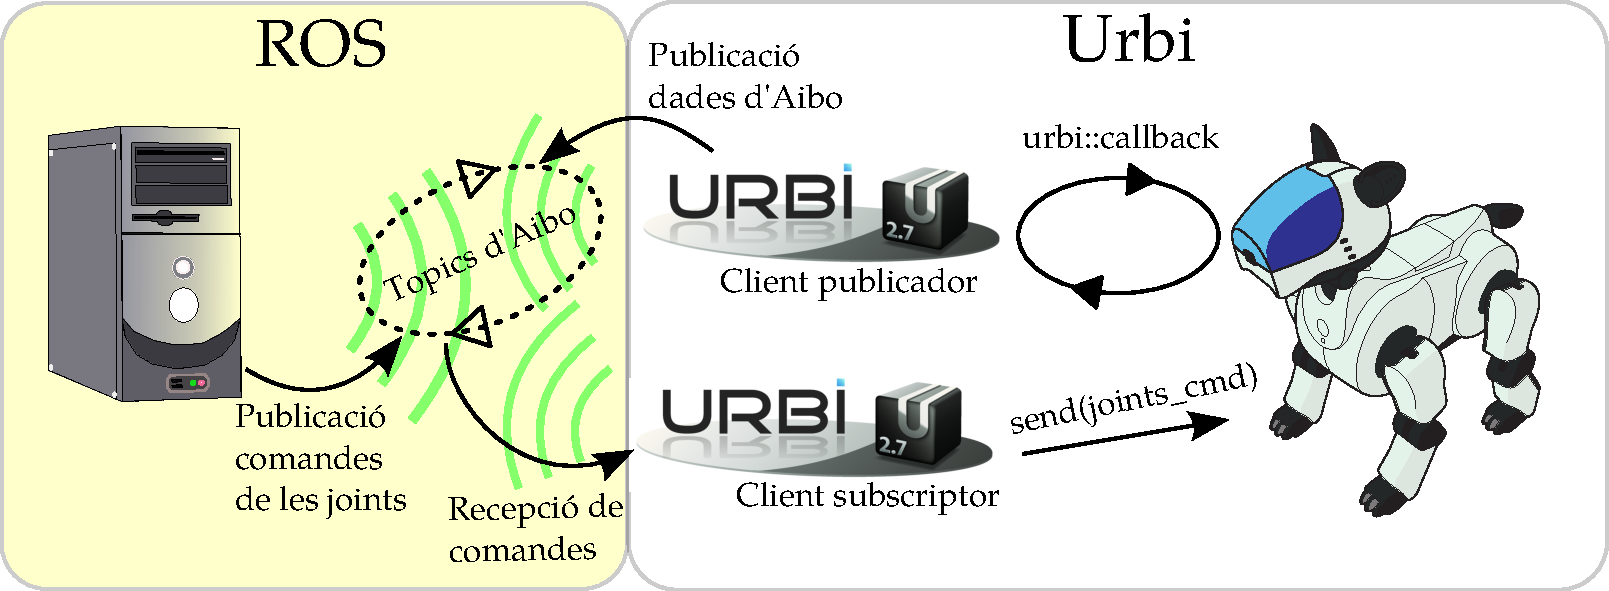
\includegraphics[width=0.95\textwidth]{Imatges/Comunicacio-ROS-Urbi-Aibo.pdf}
\caption{Comunicació entre l'AIBO, Urbi i \textit{ROS}}
\label{fig:Comunicacio-ROS-Urbi-AIBO}
\end{figure}


\subsubsection{Entre l'algorisme de control i \textit{ROS}}

\paragraph{}En parlar d'algorisme de control es refereix al codi que processa els càlculs que es requereixen per dur a terme tot el procés d'estabilització. Aquest codi és executat en un ordinador o servidor, on està instal·lat tot el \textit{software} requerit\footnote{El procés d'instal·lació està explicat en els Annexos.}. 

L'algorisme de control només depèn de \textit{ROS} per recollir la informació del conjunt acceleròmetre-giroscopi i per executar el moviment de les articulacions de l'AIBO. Per tant, el \texttt{node} d'execució és tant subscriptor del \texttt{topic} del sensor, com, alhora, és publicador del \texttt{topic} de les comandes per les articulacions.


\subsubsection{Entre el conjunt acceleròmetre-giroscopi i \textit{ROS}}

%POSAR EN ANNEXOS COM INSTAL·LAR I EXECUTAR EL ROSSERIAL
%\footnote{En els Annexos està explicada la instal·lació i l'execució}.

\paragraph{}El conjunt està connectat a l'Arduino, per tant, ha de ser aquest el que creï el \texttt{topic} on es publica la informació que ha de transmetre per \textit{ROS} a l'algorisme de control. A tal efecte existeix un \texttt{package} que permet aconseguir-ho, \texttt{rosserial}. A banda d'haver-se d'instal·lar i executar quan és el cas, també es requereix que en el codi es carreguin la llibreria \texttt{ros.h} i les corresponents al tipus de \texttt{message} al que s'hagi de subscriure o de publicar. Aquestes llibreries, juntament amb les variables que es requereixen com el \texttt{node}, el publicador i el \texttt{message}, ocupen una gran quantitat de memòria del microcontrolador i pot arribar a donar algun que altre problema, com s'explica en la Secció \ref{Calcul-posicio-inclinacio}. 

%Urbi és amb que es comunica ROS i que aquí s'ha començat a utilitzar a partir del codi que es tenia de Ricardo Téllez, pero que s'ha modificat ja que inicialment no funcionava i quan van arribar a funcionar totes ses parts s'ha mirat d'optimitzar la frequencia per tal que funcioni millor (sense aturades pero al maxim)
%Com està es tema de es codi, que fa i qui hi ha treballat amb cada part (sobretot diego, menys amb la part de camara que ha fet la Lucia), som un grup de treball que intenta que es tornin a reutilitzar els Aibos


\subsection{Estabilitat}
\label{Estabilitat}

\paragraph{}El concepte d'estabilitat és molt genèric, s'ha definit de múltiples maneres al llarg del temps, sense mai tenir una única interpretació. Dins el concepte d'estabilitat es pot diferenciar entre dues:
\begin{description}

\item[Estàtica] és aquella que assumeix que la projecció vertical del CdG està, en tot moment, dins el polígon d'estabilitat\footnote{El polígon d'estabilitat esta definit pels punts de suport del robot.} amb un marge d'estabilitat\footnote{El marge d'estabilitat assegura que per qualsevol velocitat que el robot pot arribar, no caurà degut al seu propi moment \cite{Hugel1999}.} adequat \cite{Hugel1999}.

\item[Dinàmica], en aquest cas, es tenen en compte els efectes de paràmetres dinàmics com la velocitat i l'acceleració de diferents parts del robot \cite{Yazdani2012}.

\end{description}

El fet d'estudiar l'estabilitat dinàmica es sortiria de l'abast d'aquest treball, per la seva gran complexitat, tot i existir conceptes com el \textit{ZMP}, explicat en detall en \cite{Vukobratovic2004}, que permeten aquests tipus d'estudis, fins i tot per robots bípedes. Però en aquest cas, tan sols es treballa amb l'estabilitat estàtica. Per tant, s'estableix que l'objectiu de l'algorisme de control és mantenir el CdG del robot a dintre del polígon d'estabilitat en tot moment. Aquesta tasca es podria aconseguir realitzar de diferents formes, però la majoria d'aquestes probablement queden fora de l'abast d'aquest treball. Per això, l'idea és fer-ne una aproximació, s'assumeix que la plataforma no arriba, en cap cas, a certes pendents molt elevades\footnote{Aquesta pendent màxima s'estableix en els objectius del \textit{TFG}, Secció \ref{Objectius}}.

%ANAR A PROVAR AMB S'AIBO QUE NO ESTIC SEGUR SI LI ESTIC DONANT SA MILLOR POSICIÓ POSSIBLE!!!!!

%Una de les millors formes de maxima estabilitat --> CdG retorn posicio origen. D'aqui en sortirà es dir que una altre opció no tan bona és horitzontal.

%Com definirem estabilitat, diferents mètodes...
%Explicar que s'ha proposat de fer el calcul del desplaçament del CoG, i que s'intentaria fer que aquest retornes a la posició inicial. Però finalment nomes es pot intentar que tingui horitzontalitat.
%També explicar el sistema de solucio inicial de la \textit{DMP} de com s'han de posar les potes per tal de tenir una posicio mitjanament estable.

\subsection{Algorismes de resposta davant pertorbacions}
\label{Algorismes}

\paragraph{}En la robòtica, com en qualsevol àmbit, per un mateix problema poden ser utilitzades infinitat de solucions. Ara bé, el tret característic de l'enginyeria és que d'entre la multitud de possibilitats, s'esculli la més òptima segons les condicions del moment. Abans d'optar per una opció, s'ha de tenir una idea clara del que aporta cadascuna i observar com s'adapta a la problemàtica actual.

En l'estat de l'art, s'han esmentat algunes de les possibilitats per dur a terme els objectius fixats inicialment. Aquestes opcions han estat explicades anteriorment, amb una breu descripció i trets característics que podrien ser d'interès pel nostre cas. A continuació, s'exposa com cadascuna podria adaptar-se al problema, mencionant els seus avantatges i inconvenients.

\subsubsection{Model del robot}

\paragraph{}Una de les possibilitats podria ser la creació d'un model del l'AIBO. D'aquesta forma davant una pertorbació, com és el canvi d'inclinació de la plataforma, es podria saber les accions de control que portarien el robot a l'estat desitjat.

A banda de beneficiar-se de la cinemàtica inversa\footnote{Tècnica permet determinar el moviment d'unes articulacions per portar el cos a una posició concreta}, un model permetria aplicar els algorismes, de forma virtual, en un simulador. L'algorisme simulat donaria una solució, que podria servir com a punt de partida per aplicar-ho al model físic, així la probabilitat de provocar algun risc seria molt més baixa.

\subsubsection{Aprenentatge supervisat}

\paragraph{}Per altra banda, per no continuar amb la forma típica de controlar els robots com és el fer un model, es podria utilitzar l'aprenentatge supervisat. Per tant, a partir d'un conjunt de mostres d'exemple que utilitzi com a variables explicatives l'estat del robot i com a resposta la posició final de les articulacions. Com estat del robot s'hauria d'interpretar com el conjunt de posicions de les articulacions i inclinacions, en l'eix x i l'eix y, actuals. S'han d'utilitzar tant posicions com inclinacions, ja que sinó un mateix estat tindria més d'una solució possible.

Es cert que si s'aconsegueix determinar de forma correcte l'espai de solucions, aquest model podria ser molt útil. Ara bé, hi ha cert inconvenients a l'hora de crear les mostres d'exemple segons \cite{Alpaydin2004}:

\begin{itemize}

\item Pot haver-hi impressicions en la gravació d'atributs d'entrada. En aquest cas és l'error que tenen els sensors de les articulacions i l'aparell que mesura l'angle d'inclinació.

\item Possibles errors a l'hora d'etiquetar la resposta, ja que és difícil, a banda d'infinites solucions\footnote{Existeixen infinites solucions ja que en cada pota hi ha dues articulacions que permeten desplaçar o inclinar el robot de forma longitudinal.}, encertar a mà quines han de ser les posicions exactes perquè l'AIBO es trobi horitzontal. A més, no hi ha una mesura exacta de com d'estable es troba el robot, l'únic que es té es la inclinació, però podria estar desplaçat.

\item Per últim, poden existir factors que no s'han tingut en compte, però que influeixin la resposta, com podria ser el desplaçament lateral o longitudinal, o l'acceleració.
\end{itemize}

Per la pròpia motivació que es té en el treball de voler aprendre nous coneixements, i que aquest mètode en el seu origen és fer un estudi estadístic, s'ha preferit no utilitzar-lo, tot i poder ser una eina totalment vàlida.

\subsubsection{Aprenentatge per reforç}

\paragraph{}D'entre les possibilitats que s'han plantejat fins aquí en aquest apartat, aquesta és la que més ha atret. Això és degut a que és una eina molt potent, però amb una lògica interna mitjanament simple. S'hauria de plantejar el mètode que més s'adapti al cas, i llavors crear la funció a minimitzar o maximitzar per tal de dur a terme la tasca d'estabilitat.

En aquest treball, no es té un model del robot prou acurat, per tant, es requereix d'un algorisme apta per ser utilitzat sense model. D'entre els possibles, s'escolliria el \texttt{Q-learning}, ja que és del que es disposa de més informació i, a més, l'algorisme no és molt difícil d'implementar. El \texttt{Q-learning} es basa en augmentar o disminuir la probabilitat d'una acció en un estat concret, segons el \texttt{reward} que s'ha concedit quan s'ha fet aquesta acció en aquell estat en un instant del passat\footnote{Per tant, en tornar al mateix estat hi ha més probabilitats de fer l'acció correcte, o com a mínim, menys probabilitat d'equivocar-se de nou.}.

En referència a l'acumulació de recompensa $J$, que és la funció a maximitzar o minimitzar, s'hauria d'escollir inicialment quin model utilitzar d'entre: (1) horitzó finit, (2) model de descompte o (3) recompensa mitja. Al ser l'objectiu la bondat de la posició final i que és dugui a terme en un temps determinat, el model que s'hi adapta millor és el d'\textbf{Horitzó finit}:

\begin{equation}
J=E\left\{ \sum_{h=0}^{H} R_{h} \right\}.
\end{equation}

Els algorismes d'aprenentatge per reforç es basen en gran part en l'exploració dels estats, ara bé, en un sistema com és l'AIBO existeixen massa possibles estats per poder explorar-los de forma física, a banda que són continus, i per tant, s'haurien de discretitzar per utilitzar algorismes com \texttt{Q-learning}. Per això, si s'hagués de fer s'utilitzaria l'aprenentatge de forma jeràrquica, per tal de primer només aplicar-ho a unes poques articulacions, mentre les altres estan fixes i aquestes s'afegirien de forma progressiva quan les primeres ja hagin aprés. 

Ara bé, tot i poder-se dur a terme seguint aquest procediment, és creu més convenient utilitzar algun altre mètode que convergeixi de forma més ràpida, i si escau, fer ús del \texttt{RL} per millorar el comportament del que s'hagi aconseguit.

\subsubsection{\textit{DMP}}

\paragraph{}L'algorisme de \textit{DMP} és el que s'adapta millor a la situació, ja que està dissenyat per tractar sistemes dinàmics, com és el cas. A més, té una gran robustesa davant pertorbacions, que és el que justament es necessita, considerant que el moviment de la plataforma és una pertorbació. Per altra banda, s'adapta perfectament a noves situacions, com pot ser un inici diferent al original i/o acabar en una posició que difereixi de la posició final primera.

El robot consta de diferents articulacions, cadascuna afecta d'una o altre manera el moviment del conjunt del robot. Per implementar l'algorisme, s'ha de crear una \textit{DMP} per cadascuna de les articulacions, per tant el procés d'aprenentatge s'ha de repetir tants cops com nombre juntures. En la majoria de les explicacions següents és refereix en l'aprenentatge d'una individualment, per les altres seria el mateix procés.

El primer pas que s'ha de fer, per dur a terme la DMP, és tenir un moviment original. Aquest és podria extreure, com s'ha explicat en l'apartat \ref{DMP-estat-de-l'art}, a partir de: (1) imitació, (2) demostració amb el propi robot, (3) trajectòria programada. D'entre les tres, s'ha escollit la tercera, ja que les articulacions de l'AIBO són \textit{PIDs} i, per tant, la posició que se li programi és segur que es durà a terme. A més, la imitació no tindria sentit, si no hi ha un altre robot a imitar, i la demostració no és una bona opció, perquè a banda de ser impossible donar el moviment a totes les articulacions alhora de forma manual, tampoc seria precís.

Havent escollit el mètode per donar el moviment original, s'ha de saber com ha de ser aquest. Un tipus de trajectòria molt utilitzat és la de mínim \texttt{jerk}\footnote{\texttt{Jerk} és la derivada de l'acceleració}. Aquesta és una trajectòria suavitzada calculada a partir d'una posició inicial, final i el temps requerit per arriba-hi, minimitzant el \texttt{jerk}. Es deixen els detalls d'aquest tipus de trajectòria per \cite{Shadmehr2004}.

Un cop es té la trajectòria, a partir d'aquesta es poden extreure els pesos $w_i$ aproximant mínims quadrats amb gaussianes i, per tant, la funció no lineal $f(s)$ queda definida amb una primera solució, figura \ref{fig:LdF-trajectories}. Amb tan sols aquesta primera solució és factible el dur a terme les \textit{DMPs} de forma correcta. Ara bé, en el treball és desitja que s'arribi a la posició de màxima estabilitat de la forma més precisa. Per això, s'han de poder modificar els pesos $w_i$ i el $goals$ de les articulacions, de tal manera que la posició final sigui l'adequada. Una bona opció és l'algorisme $\mathrm{PI^2}$, que et permet millorar tan els pesos, com els $goals$ depenent de paràmetres externs a la dinàmic del sistema, com podria ser el desplaçament del CdG o la inclinació. 
\begin{figure}[tb]
\centering
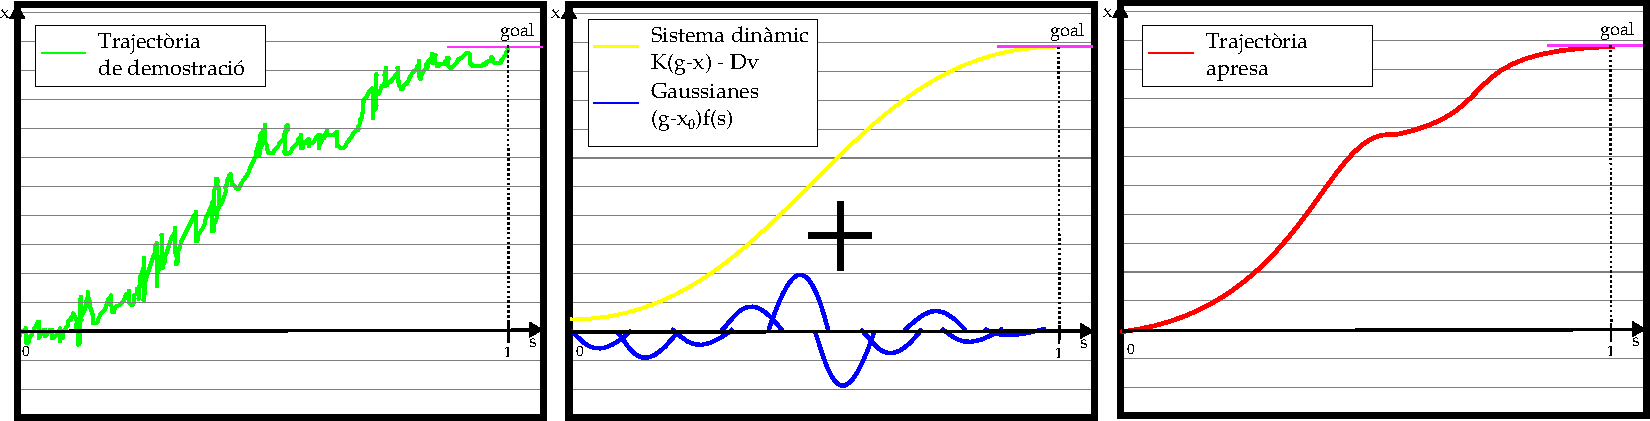
\includegraphics[width=0.97\textwidth]{Imatges/Aprenentatge-per-demostracio.pdf}
\caption[\textit{DMP} a partir una trajectòria de demostració]{Donada una trajectòria de demostració (esquerra), aquesta és aproximada a partir de la suma del sistema dinàmic, definit per $K$ i $D$ preestablertes, i d'unes gaussianes (centre), que són les que s'han aproximat per mínims quadrats. La suma resulta en la trajectòria apresa (dreta).}
\label{fig:LdF-trajectories}
\end{figure}

%Explicar que és i despres dir quan la combinacio amb PI² que el que provoca es una unió entre DMP i aprenentatge per reforç

%\subsubsection{Affordance}
%Affordance: Mes o menys es podria entendre com els sensors i actuaduadors serien moduls neuronals que envien informació ja filtrada als altres moduls neuronals de tal manera que vagi enfocat a fer una tasca determinada

\subsubsection{Elecció final}
\paragraph{}En conclusió, el mètode utilitzat és la \textit{DMP} conjuntament amb l'algorisme $\mathrm{PI^2}$. Per una banda, la \textit{DMP} dona una solució inicial bastant encertada\footnote{La bondat d'aquesta solució depèn de la qualitat del $goal$ per les articulacions que s'ha estimat.}. Per l'altra banda, el $\mathrm{PI^2}$ millora tant els pesos com els $goals$ de les articulacions, depenent dels paràmetres externs com són el desplaçament del CdG o la inclinació del robot.

%Explicar que es finalment s'escull per les DMPs juntament amb PI² que donarà la part de reinforcement learning que es necessita per tal de poder dur a terme el treball de la forma més adient possible, ja que aquesta part corregirà l'error que comet el goal de la DMP.

\subsection{Codis amb \textit{DMPs} implementades}
\label{codis-amb-DMPs-implementades}

\paragraph{}La creació de l'algorisme de \textit{DMPs} és un fet que no troba dins l'abast del treball, degut a la gran complexitat d'aquest. Està basat en equacions diferencials, canvis de variables, ús de Gaussianes, aproximacions per Fourier o per mínims quadrats, etc. Per una banda, estaria la dificultat de crear el codi, però més complicada és el treball que porta el depurar-lo. Per això, s'ha optat per cercar codis que portin implementades les \textit{DMPs}, d'entre els que s'han trobat només s'han plantejat els dos que es troben a continuació perquè són uns dels que utilitzen la \textit{DMP} modificada que s'ha plantejat en l'apartat \ref{DMP-estat-de-l'art} de l'estat de l'art.
%Es molt complex el fer el codi per implementar les DMPs ja que són un seguit d'equacions diferencials amb transformacions de variables, us de Gaussianes, etc.
%Per això s'implementa a partir de codis ja existents que funcionen, pero adaptant-lo al cas de treball.
\subsubsection{\textit{DMPs} de Scott Niekum}

\paragraph{}El package creat per Scott Niekum està basat en l'article \cite{Pastor2009}. Inicialment, s'ha optat per aquest codi perquè és senzill i útil, figura \ref{fig:diagrama-sniekum}. S'ha estudiat el seu funcionament, on a diferència de l'algorisme explicat en l'apartat \ref{DMP-estat-de-l'art}, aquest l'aproximació es fa amb $Fourier$, en lloc d'utilitzar $gaussianes$. Aquest codi crea les \textit{DMPs} sense problemes, com s'ha demostrat en \cite{Pfeiffer2014}, però té el problema que no porta implementat cap tipus d'algorisme de millora de la política a partir de paràmetres externs a la pròpia dinàmica del sistema. Per això, s'ha preferit utilitzar el \texttt{package} que s'explica a continuació.

\begin{figure}[tb]
\centering
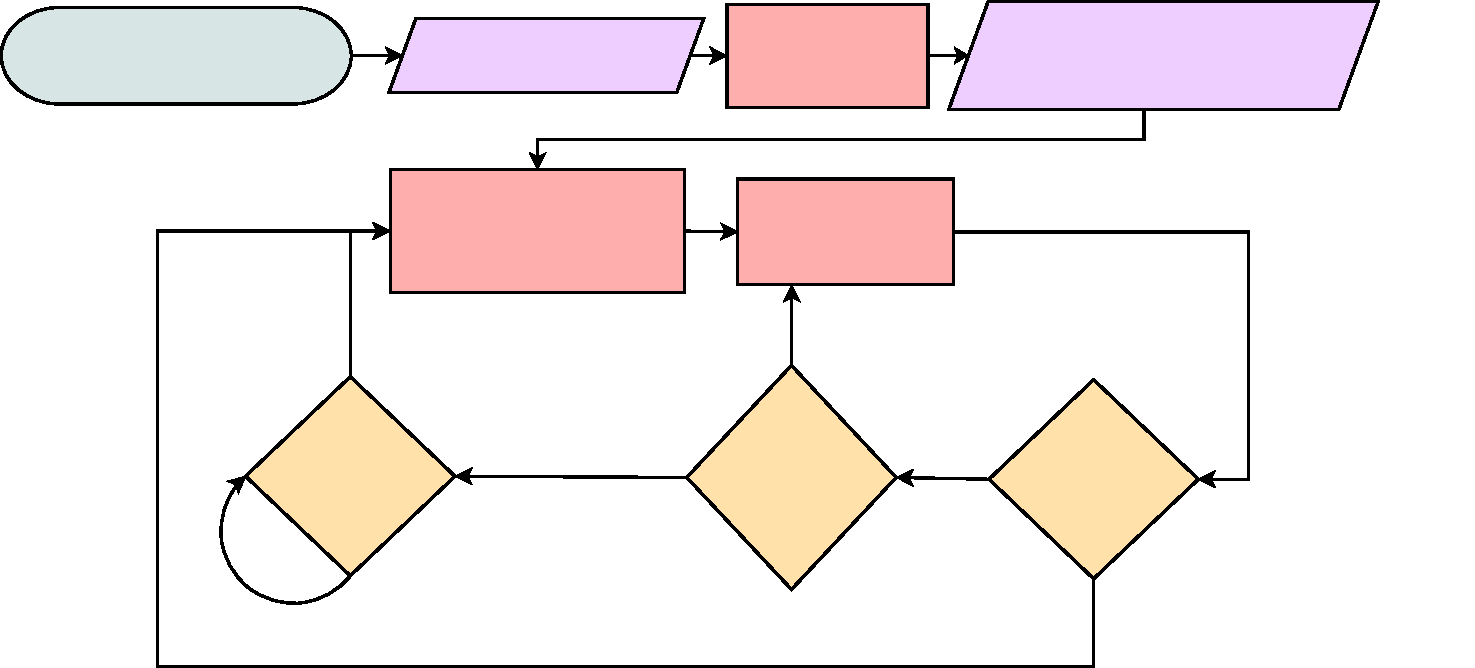
\includegraphics[width=0.95\textwidth]{Imatges/diagrama-sniekum.pdf}
\caption[Diagrama fluxos del codi de Scott Niekum]{Diagrama de fluxos del suposat funcionament en aquest cas del codi de Scott Niekum.}
\label{fig:diagrama-sniekum}
\end{figure}

%Prenen com a codi original el de les dmps del package de ROS de DMP, creat per ell mateix, i l'implementa en robots en aquest package. Esta basat en el document ICRA2009 de Peter Pastor http://www-clmc.usc.edu/publications/P/pastor-ICRA2009.pdf
%Es sencill i útil, va directe al gra, ara té el problema que no té implementat per posar-hi aprenentatge per reforç, la qual cosa és molt important per aquest projecte. Inicialment es va estudiar a fons el funcionament d'aquest codi i observar com es podria arribar a implementar en el cas actual, finalment es va veure que amb aquest codi no es podia implementar o seria complicat de posar l'algorisme de PI².

\subsubsection{Package complert del robot PR2 del \textit{USC-CLMC}}
\label{Package-USC-CLMC}

\paragraph{}A continuació es presenta un conjunt de  \texttt{packages} públics, es poden trobar en aquesta web \cite{USC-CLMC-package} del \textit{USC-CLMC} (\textit{\textbf{C}omputational \textbf{L}earning and \textbf{M}otor \textbf{C}ontrol \textbf{L}ab at the \textbf{U}niversity of \textbf{S}outhern \textbf{C}alifornia}). Aquests permeten l'ús de les DMPs amb l'algorisme $\mathrm{PI^2}$, en el robot PR2 de Willow Garage \cite{Bohren2011}, incloent el control en temps real per interfície gràfica, l'ús de percepció auditiva, etc. Per tant, ha hagut de ser adaptat al cas del treball, enfocat per l'AIBO i amb molts menys complements. Per fer-ho s'han eliminat molts dels \texttt{packages} que s'hi inclouen, perquè no s'han d'utilitzar. A més, s'ha hagut de crear un codi d'execució, perquè realment el \texttt{package} és la base sobre la que pot funciona l'algorisme, però es necessita un codi que l'engegui. 

El fet d'eliminar els \texttt{package} pot semblar una tasca fàcil, però al darrera hi ha hagut un gran treball d'entendre un conjunt de codis, creats per altres persones i de tal magnitud. Per altra banda, a mesura que s'ha avançat en el coneixement del conjunt del \texttt{package} i en la creació del codi d'execució, s'ha anat modificant el conjunt per permetre el funcionament global. En aquest apartat, inicialment s'explica els trets més importants dels \texttt{packages} que finalment s'han utilitzat, i cap el final s'esmenten alguns dels canvis respecte el codi original i el perquè d'aquests.

\vspace{20pt}
\textbf{\textit{DMP}}

El \texttt{package} de les \textit{DMPs} és nucli de l'algorisme. En la seva base funciona de la mateixa forma que el codi presentat anteriorment de Scott Niekum, ara bé, canvia en que la comunicació amb el propi codi és fa des de \textit{ROS}. D'aquesta manera permet modificar els paràmetres de la DMP sense la necessitat de modificar el codi, sinó que és pot fer modificant les propietats del node d'execució\footnote{Això és pot fer amb la comanda \texttt{node$\_$handle.setParam("nom$\_$paràmetre", valor$\_$paràmetre)} o amb \texttt{usc$\_$utilities::write(node, "nom$\_$paràmetre", valor$\_$paràmetre)} si és un vector.}. En el codi d'execució d'aquest treball aquests paràmetres estan donats de forma automàtica dins el codi. Una altre gran avantatja de la comunicació mitjançant \textit{ROS} és el poder publicar l'estat de la \textit{DMP} en tot moment a través d'un \texttt{topic} i la facilitat d'intercanviar informació amb l'exterior.



%SI ES FINAL NO ES DIU ES PERQUE AÇO S'HAURA DE MODIFICAR

%Aqui es troben tots els diferents codis que utilitza l'USC-CLMC (Computational Learning and Motor Control Lab at the University of Southern California). 
%PACKAGES QUE HI HA I MITJANAMENT FUNCIONAMENT
%Aquest package apart de ser pel robot PR2, confia en que es té un model del propi robot (per tant el robot sap on es troba en cada instant), utilitza aprenentatges que no es necessiten, utilitza cinematica inversa, visualització amb gui dels parametres, reconeixement i reproduccio d'audio i un llarg etcètera. Es per això que s'ha hagut de reduir molt i nomes quedar-se amb l'essencial que és:
%DMPs (d'aquest s'ha tret tot el relacionat amb la propia demostracio ja que aquí s'impleneta a traves de codi i no pas desplaçant el propi robot, el controlador que envia les ordres de moviment al robot ja que aqui van a traves de ROS i es un sistema totalment diferents (tot i que s'ha pres com a referencia el que estava fet) i la visualitzacio en gui)
%el learning_policy (que és en essència el PI², d'aquí l'únic que s'ha tret ha estat algun tipus de policy que no era la que s'utilitzava per les dmps i algun test que no era necessari).
%La part que s'ha deixat ha hagut de ser modificada en molts punts per tal que s'adaptes al nostre cas, aquests canvis i l'explicació del funcionament s'expliquen més endavant.

\newpage
\section{Disseny}

\paragraph{}Inicialment, s'ha plantejat un disseny amb un model del robot que serviria per simular tot el conjunt amb l'ordinador. D'aquí en sortiria un solució inicial per implementar al robot físic, i a partir d'aquest arribar a la solució final. La solució primera estalviaria possibles perills, tant pel propi robot com per l'entorn, i ajudaria a aconseguir la convergència a una solució final més ràpidament. En referència a les \textit{DMPs}, com s'ha explicat en l'apartat \ref{Package-USC-CLMC}, el codi utilitzat és el creat per \textit{USC-CLMC}, però modificat per l'adaptació a aquest treball. Ara bé, aquest dona dues opció d'execució a escollir segons l'algorisme: (1) \textit{DMPs} conjuntament amb l'algorisme $\mathrm{PI^2}$, (2) \textit{DMPs} sense el $\mathrm{PI^2}$; el funcionament dels dos tipus es troben explicats en aquest mateix apartat. Per altra banda, en aquest apartat també s'explica l'ús del conjunt acceleròmetre-giroscopi, en l'algorisme de control, i de influència i control de la plataforma.

%SI ES FINAL NO ES CONTROLA SA PLATAFORMA S'HA DE MODIFICAR AÇO.

%ON FICAR MODIFICACIONS FETES AL CODI DEL USC-CLMC??? AQUI O QUAN INTRODUESC EL CODI EN L'ESTUDI PRELIMINAR??

%Explicació general com queda finalment, que s'agafa les DMPs amb el PI², l'ús del accelerometre, explicar quin seria el reward, el goal de la DMP inicialment, etc. Explicar el funcionament global del conjunt com afecta cada cosa etc. Amb això s'hauria d'entendre que és el meu treball
%Després sub apartats amb explicacions exteses de cada cosa

\subsection{Model de l'Aibo}
%EXPLICAR TOT TOT LO DE ES MODEL
%Dir que tot i que després de la solucio inicial s'ha de seguir fent aprenentatge ja que el model no és perfecte i per tant té un cert error, que quan es posa en el robot físic aquest error es corregirà.


\subsection{Moviment del centre de gravetat}

%ABANS D'AQUEST APARTAT S'HA D'HAVER PARLAT SOBRE:
%Una de les millors formes de maxima estabilitat --> CdG retorn posicio origen. D'aqui en sortirà es dir que una altre opció no tan bona és horitzontal.

%Es pensava utilitzar l'acceleròmetre del pròpi Aibo, a partir d'observar les mostres que es donaven es va comprovar com l'error era molt gran i per això es va comprar un accelerometres més precis MPU6050. Apart d'això també es fiava de treure el desplaçament del CoG (apart d'obviament l'angle d'inclinacio del robot).

\paragraph{}Tal i com s'ha vist al llarg del treball, uns dels requisits per poder aconseguir recuperar l'estabilitat és tenir les mesures dels moviments del robot. Com a idea inicial, s'ha pensat utilitzar el sensor triaxial d'accelerometria que porta incorporat el propi AIBO, i d'aquesta forma poder estudiar el moviment d'aquest. Però abans s'han fet unes comprovacions de la fiabilitat de les dades d'aquest sensor. Aquestes comprovacions es basen en l'observació de la variabilitat de les mesures i comprovar si l'angle d'inclinació extret a partir de l'acceleració és el mateix que el mesurat externament. Finalment ha resultat que no és gens precís per la tasca que ha de desenvolupar.

\subsubsection{Acceleròmetre MPU6050 i giroscopi GY-521}

\paragraph{}Al no ser el sensor del propi robot d'utilitat en el treball, s'ha decidit comprar un altre sensor triaxial d'accelerometria amb un giroscopi de tres eixos. En aquest cas, s'ha optat per una peça on hi ha integrat l'acceleròmetre \texttt{MPU6050} i el giroscopi \texttt{GY-521}. S'ha escollit aquest, en primera instancia, perquè està enfocat per a ser utilitzat amb Arduino, que és un microcontrolador del que es disposa en el departament i que ja es pensa utilitzar per altres motius. A més, existeix molta informació per la xarxa, com llibreries\footnote{Entre d'elles un de les més utilitzades i molt pràctica és la \texttt{i2cdevlib}, on a banda de per aquest conjunt acceleròmetre-giroscopi, també n'hi ha per molts altres \cite{Rowberg}} o aplicacions fetes, a banda de ser recomanat per la seva qualitat-preu.

%IDEA: HAGUES POGUT ENVIAR PER ROS LA INFORMACIO DE L'ACCELEROMETRE I GYRO I FER EL FILTRE A L'ORDINADOR, PERO HAVES ESTAT PRACTICAMENT EL MATEIX, I PER COMODITAT D'ESTAR JA IMPLEMENTAT S'HA ESCOLLIT EL PRIMER MÈTODE, PERÒ PODRIA SER UNA PROVA A FER PER MILLORAR-NE LA QUALITAT. TOT I QUE D'AQUESTA FORMA HAGUES POGUT UTILITZAR EL FILTRE KALMAN, INCONVENIENT--> S'HA DE TENIR UN THREAD NOMÉS PEL CALCUL

Ara bé, el fet de formar part de l'AIBO crea la problemàtica d'haver d'implementar una comunicació entre el sensor i l'algorisme de control. Com que és té un entorn de treball, \textit{ROS}, que ja s'està utilitzant per comunicar-se amb l'ordinador, és pot aprofitar aquest entorn per tal d'incorporar la informació que es vulgui enviar al robot. 

A partir de l'acceleròmetre es treu informació de les acceleracions que pateix aquest sensor, incloent la gravetat, aquest transmet les dades en RAW que s'han de dividir per $16384$ per a ser transformats a $G$s\footnote{Força $G$, per tant, el resultat de la divisió s'ha de multiplicar per $9,80665$ per passar-ho a $m/s^2$.}. Per altra banda, el giroscopi mesura la velocitat angular, abans d'utilitzar les dades que arriben directament d'aquest, s'ha de passar del RAW a \textit{º/s} (graus per segon) dividint-ho $131$.

\subsubsection{Càlcul de la posició i de la inclinació}
\label{Calcul-posicio-inclinacio}

\paragraph{}Com s'ha explicat en l'apartat \ref{Estabilitat} d'Estabilitat, una de les millors formes de cercar la màxima estabilitat, dins l'abast del \textit{TFG}, és provocar que el CdG retorni a la posició d'origen. Per tant, es requereix saber en tot moment quan s'ha desplaçat respecte aquest origen, però per això es necessita tenir la informació de la inclinació del robot, per tal d'extreure tan sols la component de l'acceleració que ens interessa.


\vspace{20pt}
\textbf{Càlcul de la inclinació}

En aquest càlcul, es requereix essencialment del giroscopi, perquè tant sols s'han d'integrar les dades subministrades per aquest. L'acceleròmetre només podria ser servir, per extreure la inclinació, si s'estigués estàtic o, com és en aquest cas, per ajudar a filtrar les dades. Per tal de dur a terme aquest filtre, s'han trobat dos tipus de filtres que podrien ser útils, el filtre \texttt{Kalman} i el filtre \texttt{complementari}.

El filtre Kalman es basa en l'estimació de l'estat del sistema a partir de la informació de l'acceleròmetre i el giroscopi, en el moment anterior i en l'actual. Per altra banda, el filtre complementari és basa en l'ús de les dades del giroscopi, per la mesura en temps curts, i realitzar la correcció de la deriva, amb les dades de l'acceleròmetre \cite{Gaydou2011}. Un filtre complementari és un filtre Kalman, però en unes condicions i restriccions determinades. Per això no difereixen gaire en els resultats donats, el Kalman és més precís, però requereix de més recursos computacionals.

Inicialment, s'ha plantejat utilitzar el filtre Kalman, per això s'ha pres el codi de \cite{Lauszus2012}, on està l'algorisme del Kalman i del filtre complementari fets en un exemple per Arduino. El problema ha sorgit en intentar implementar tot el conjunt de filtre Kalman i les llibreries que permeten la comunicació de l'\textit{Arduino Uno} amb \textit{ROS}, perquè la placa no té prou memòria per abarcar-ho tot. Pel que sembla, la llibreria de \textit{ROS} ocupa pràcticament la meitat de la memòria del microcontrolador i la resta no és suficient per l'algorisme del filtre Kalman, tot i haver intentat optimitzar al màxim l'ús de memòria.

Una opció per solucionar el problema anterior hagués pogut ser transmetre per \textit{ROS} tan sols les dades RAW dels sensors, i llavors fer el filtratge en l'ordinador, però s'hauria de tenir un procés més en paral·lel. Però s'ha cregut més convenient utilitzar el filtre complementari, que com s'ha dit requereix de menys recursos computacionals i s'ha provat que si que pot implementar tot el conjunt.

El filtre complementari matemàticament és molt simple \eqref{eq:filtre-complementari}, tant sols depèn d'un paràmetre $\lambda$ que determina quin percentatge es pren de l'angle calculat amb l'acceleració i la resta pel giroscopi. Ara bé, per tal de poder ser útil s'hi han hagut de fer algunes millores:

\begin{itemize}
\item Les dades que s'utilitzen són una mitja de quinze mostres RAW
\item Només varia la publicació a \textit{ROS} si la diferència entre l'angle anterior i l'actual és major a 0,02 º
\end{itemize}

\begin{equation} 
\theta_{compl} = (1 - \lambda)(\theta_{compl} + w_{giro}\mathrm{d}t) + \lambda \theta_{accel} \label{eq:filtre-complementari}
\end{equation}

\begin{figure}[tb]
\centering
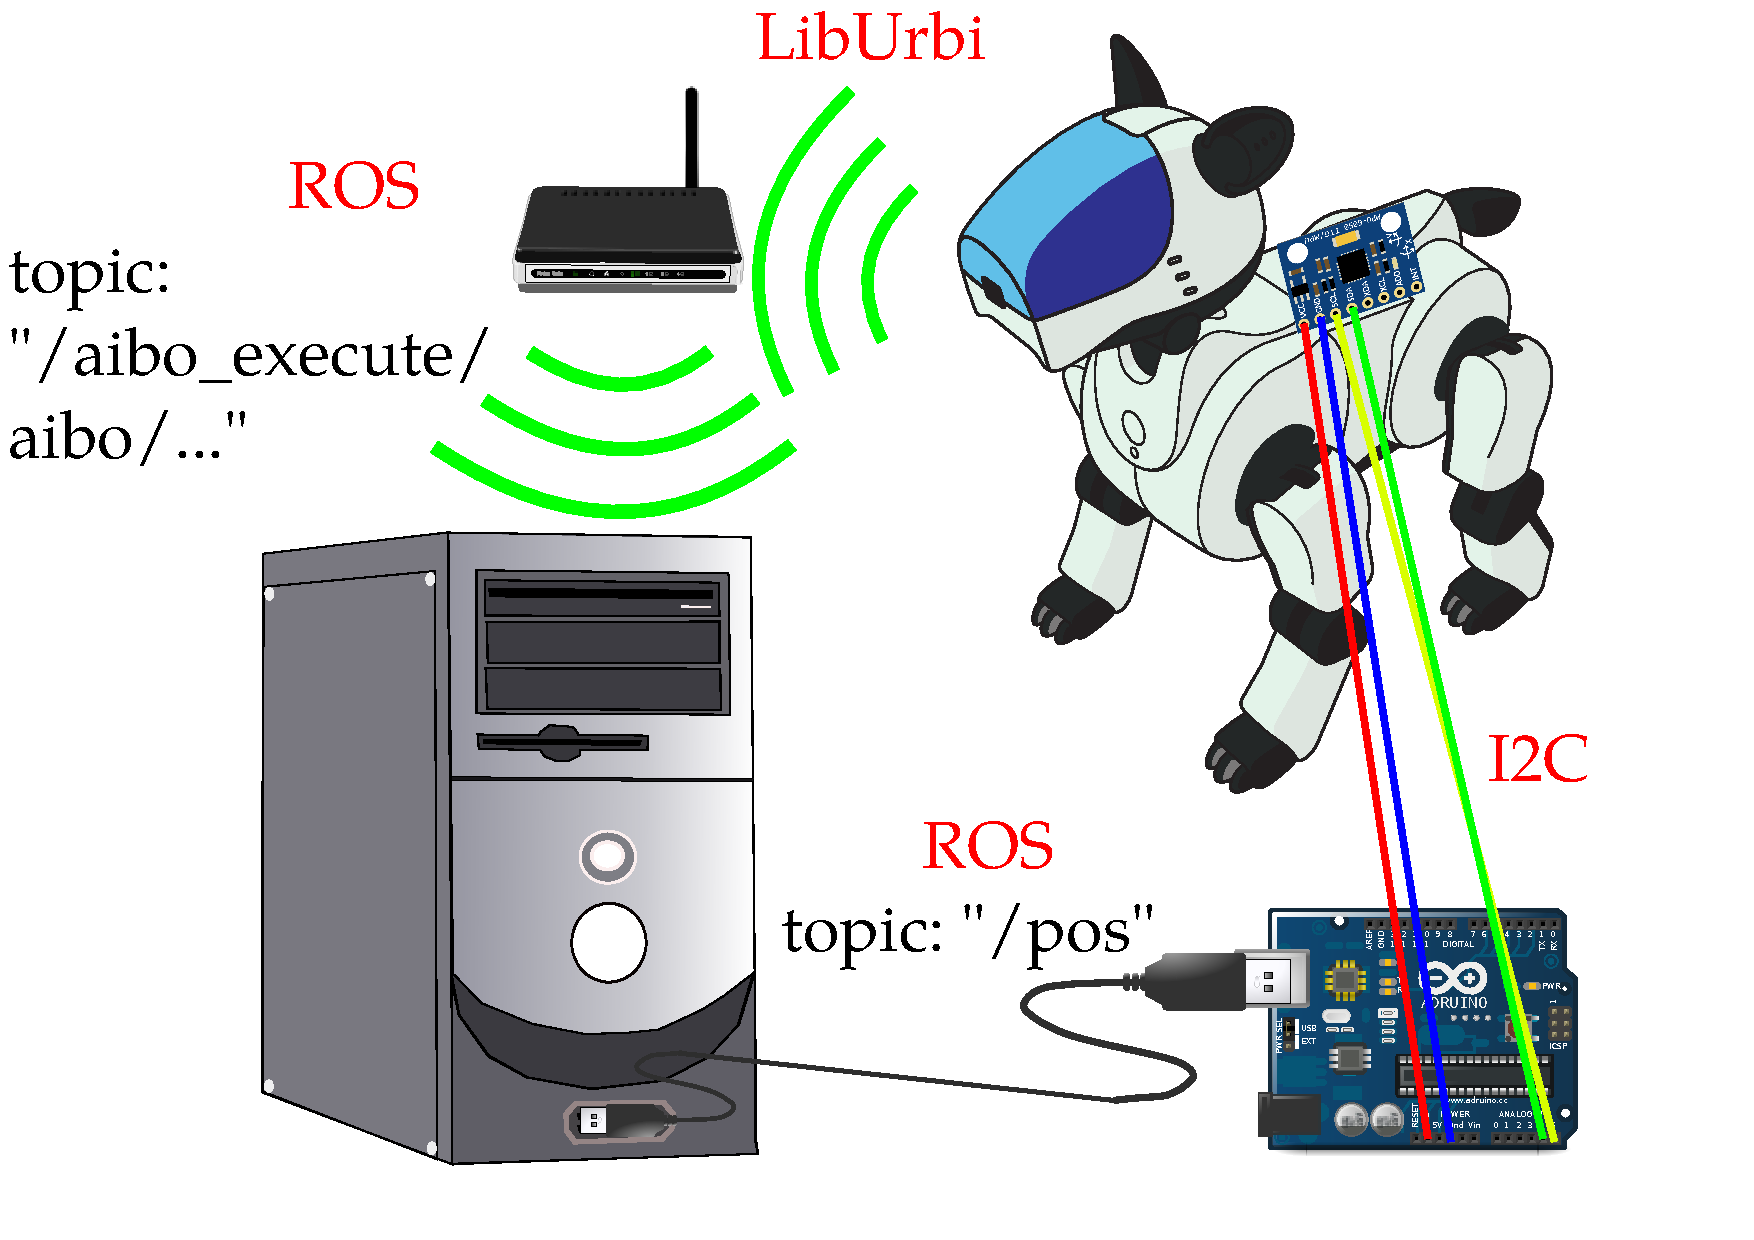
\includegraphics[width=0.8\textwidth]{Imatges/esquema-comunicacio-ROS-Aibo-ordenadora.pdf}
\caption{Esquema de connexions entre AIBO-\textit{ROS} i sensor-Arduino-\textit{ROS}}
\label{fig:connexions-Aibo-ROS-sensor-Arduino-ROS}
\end{figure}

%Arduino és compatible amb tota la família Arduino, amb l'excepció de l'\textit{Arduino Mega} i l'\textit{Arduino Leonardo} que s'han de desactivar els \texttt{pull-ups} de les entrades. Per això no s'ha utilitzat l'\textit{Arduino Mega} que es té en el departament, sino un \textit{Arduino Uno} prestat per un company.

\subsection{Plataforma}
%Funcionament de la plataforma, com esta connectada a l'Arduino i alimentació i que és el que li faig fer.
%Suposadament si s'estés utilitzant el PI² s'hauria de quedar fixa en una posició, ara bé, com que està implementat les DMPs i tan sols esta aprenent de la demostració, es pot moure en diferents direccions i l'Aibo es va adaptant a la inclinació.

\subsection{Execució \textit{DMPs} sense $\mathrm{PI^2}$}
%Explicacions i esquema de blocs del codi i funcionament de les DMPs 
\subsection{Execució \textit{DMPs} amb $\mathrm{PI^2}$}
%On es que afecta el PI² explicat tant amb paraules com esquemes de blocs


\newpage
%Abans d'això he de posar PRESSUPOST?? Realment gastat només he gastat amb l'accelerometre la resta ha estat gratuït...
%PLANIFICACIO TEMPORAL??
%I IMPACTE MEDI AMBIENTAL??
\section{Conclusions}

\newpage
\section*{Agraïments}
\addcontentsline{toc}{section}{Agraïments}

\newpage



\bibliography{./Bibliografia/library}
\addcontentsline{toc}{section}{Referències}
\label{Referencies}


\appendix
\clearpage % o \cleardoublepage
\addappheadtotoc
\appendixpage

\section{Instal·lació de \textit{ROS}, llibreries d'Urbi i paquet aibo$\_$server}

\paragraph{}Tot seguit es mostren els passos a seguir per tal d'instal·lar \textit{ROS} i com afegir una carpeta al la variable \texttt{ROS$\_$PACKAGE$\_$PATH}\footnote{Aquí es troben les direccions de les carpetes on \textit{ROS} cerca els \texttt{packages}.}.

\begin{enumerate}

\item Preparar per instal·lar \textit{ROS} (en aquest cas per Ubuntu 12.04 32 bits).

\texttt{sudo sh -c 'echo "deb http://packages.ros.org/ros/ubuntu precise main" \\> /etc/apt/sources.list.d/ros-latest.list'}

\item Configurar claus de \textit{ROS}.\\
\texttt{wget http://packages.ros.org/ros.key -O - | sudo apt-key add -}

\item Instal·lar \textit{ROS fuerte}.

\texttt{sudo apt-get update}\\
\texttt{sudo apt-get install ros-fuerte-desktop-full}

\item Per tal que els \texttt{packages} en la carpeta del propi \textit{ROS} puguin ser trobats més còmodament. La comanda final és per poder seguir treballant en el mateix terminal.

\texttt{echo "source /opt/ros/fuerte/setup.bash" $\gg$ $\sim$/.bashrc\\source $\sim$/.bashrc}

\item Es necessiten instal·lar alguns paquets per poder continuar, com és el \texttt{rosws}, que es part del paquet \texttt{rosinstall}.

\texttt{sudo apt-get install python-rosinstall python-rosdep}

\item Es crea una carpeta de treball, extensió de la propia de \textit{ROS}.

\texttt{rosws init $\sim$/fuerte /opt/ros/fuerte}\\
\texttt{mkdir $\sim$/fuerte/sandbox}\\
\texttt{rosws set ~/fuerte/sandbox}

\item Per acabar la instal·lació de \textit{ROS}, es repeteix l'acció (4), però en aquest cas, per poder ser trobats els \texttt{packages} de la carpeta que s'ha creat.

\texttt{echo "source $\sim$/fuerte/setup.bash" $\gg$ $\sim$/.bashrc\\source $\sim$/.bashrc}

\item Tot seguit, s'ha d'instal·lar la llibreria d'urbi. En aquest cas, tan sols s'ha descarregar l'arxiu comprimit\footnote{\url{http://www.gostai.com/downloads/urbi/1.5/urbi-sdk-1.5-l0258c7a-i486-linux-gnu-gcc-4.1.tar.gz}} i extreure'l en \textbackslash .


\item Finalment per instal·lar el paquet aibo$\_$server, s'ha de copiar la carpeta en alguna de les direccions de \texttt{ROS$\_$PACKAGE$\_$PATH} i compilar seguint aquest procediment:

\texttt{roscd aibo$\_$server/}\\
\texttt{rosmake --pre-clean}

\end{enumerate}

\section{Bibliografia}

\end{document}  